\documentclass{article}


\usepackage{PRIMEarxiv}

\usepackage[utf8]{inputenc} % allow utf-8 input
\usepackage[T1]{fontenc}    % use 8-bit T1 fonts
\usepackage{hyperref}       % hyperlinks
\usepackage{url}            % simple URL typesetting
\usepackage{booktabs}       % professional-quality tables
\usepackage{amsfonts}       % blackboard math symbols
\usepackage{nicefrac}       % compact symbols for 1/2, etc.
\usepackage{microtype}      % microtypography
\usepackage{lipsum}
\usepackage{fancyhdr}       % header
\usepackage{graphicx}       % graphics
\graphicspath{{media/}}     % organize your images and other figures under media/ folder


\usepackage{tikz}
\usepackage{tikz-cd}
\usepackage{subcaption}
\usetikzlibrary{matrix}
\usepackage{graphicx}
\usepackage{pgfplotstable}
\usepackage{amssymb}
\usepackage{mathtools}
\usepackage[utf8]{inputenc}
%\usepackage[english]{babel}
\usepackage{amsmath} 
\usepackage{amsthm}
\usepackage{algorithm}
\usepackage{algpseudocode} 
\usepackage{hyperref}
\usepackage{wrapfig}
\usepackage{pgfplots}
\usepackage{adjustbox}
\usepackage{caption}
\usepackage{multicol}
\usepackage{booktabs}
\usepackage{caption}
\usetikzlibrary{automata,arrows,positioning,calc}
\usetikzlibrary{shapes.geometric, arrows.meta, positioning}
\usepackage[utf8]{inputenc}
\usepackage[T1]{fontenc}
% \usepackage[numbers,sort&compress]{natbib}
%\usepackage{url}

\usepackage{xcolor} % for color support
\usepackage{hyperref}
\let\Bbbk\relax
\usepackage{cleveref}
\usepackage{fontawesome5}
\usepackage{mwe} % Minimum working example
\usepackage{pgfplots}
\usepackage[numbers,sort&compress]{natbib}

\newcommand{\weight}{\mathcal{w}}
%\newcommand{\ngh}{\textsf{$N_{G_}^e}$}
\newcommand{\nedges}{\mathcal{N}_T}
\newcommand{\tim}{\mathsf{\tau}}



%Header
\pagestyle{fancy}
\thispagestyle{empty}
\rhead{ \textit{ }} 

% Update your Headers here
\fancyhead[LO]{Classification of Temporal Graphs using Persistent Homology}
\fancyhead[RE]{S. Pritam, R. Roy and M.C. Sajeev} % Firstauthor et al. if more than 2 - must use \documentclass[twoside]{article}



  
%% Title
\title{Classification of Temporal Graphs using Persistent Homology
%%%% Cite as
%%%% Update your official citation here when published 
%\thanks{\textit{\underline{Funding: All three authors are partially supported by a grant from Fujitsu Limited.}}}
%\textbf{Authors. Title. Pages.... DOI:000000/11111.}} 

}
\author{
  Siddharth Pritam \\
  Chennai Mathematical Institute, India \\
  \texttt{spritam@cmi.ac.in} \\
  %% examples of more authors
   \And
  Rohit Roy \\
  Chennai Mathematical Institute, India \\
  \texttt{rohitroy@cmi.ac.in} \\ 
  \And
  Madhav Cherupilil Sajeev \\
  Institut Polytechnique de Paris, France \\
  \texttt{madhav.cherupilil-sajeev@polytechnique.edu} \\
  %% \AND
  %% Coauthor \\
  %% Affiliation \\
  %% Address \\
  %% \texttt{email} \\
  %% \And
  %% Coauthor \\
  %% Affiliation \\
  %% Address \\
  %% \texttt{email} \\
  %% \And
  %% Coauthor \\
  %% Affiliation \\
  %% Address \\
  %% \texttt{email} \\
}


\begin{document}
\maketitle


\begin{abstract}
  Temporal graphs effectively model dynamic systems by representing interactions as timestamped edges. However, analytical tools for temporal graphs are limited compared to static graphs. We propose a novel method for analyzing temporal graphs using Persistent Homology. Our approach leverages $\delta$-temporal motifs (recurrent subgraphs) to capture temporal dynamics %without aggregation
  . By evolving these motifs, we define the \textit{average filtration} and compute PH on the associated clique complex. This method captures both local and global temporal structures and is stable with respect to reference models. We demonstrate the applicability of our approach to the temporal graph classification task. Experiments verify the effectiveness of our approach, achieving over 92\% accuracy, with some cases reaching 100\%. Unlike existing methods that require node classes, our approach is node class free, offering flexibility for a wide range of temporal graph analysis.

\end{abstract}

% keywords can be removed
\keywords{Temporal graph \and Persistent Homology.}


\section{Introduction}
Graphs or networks provide a versatile framework for analyzing complex systems, representing entities as nodes and their relationships as edges. They capture the structural connectivity or topology of a network, characterized by measures such as degree distribution, motifs (recurring subgraphs), connected components and  cycles (\textit{homology classes}). These metrics form the basis for understanding the underlying system. Since many real-world systems are dynamic, \textit{temporal graphs}~\cite{Holme2012} are well-suited for modeling such systems, representing interactions as timestamped edges. Applications range from ecological networks to human close-range interactions, collaboration networks, biological signaling networks~\cite{Holme2012, eagle2009inferring, cattuto2010dynamics, barrat2013empirical,stopczynski2014measuring, BravoHermsdorff2019}.

%Temporal graphs encapsulate the evolving `temporal connectivity' of a network. A fundamental concept in this context is \textit{reachability}: given two temporal edges \(uv\) and \(vw\) with timestamps \(t_1\) and \(t_2\), where \(t_1 < t_2\), one can traverse from \(u\) to \(w\) via \(v\), but not the reverse. This temporal aspect introduces complexities that go beyond static graph analysis.

The analysis of static graph topology is well-developed, with various metrics and tools designed to assess key properties. While some of these metrics, such as path-length, centrality, and betweenness, have been extended to temporal graphs~\cite{Holme2012}, fewer tools exist for analyzing temporal graphs. Existing methods often aggregate temporal data into discrete time-window snapshots~\cite{Araujo2014, Dunlavy2011, tinarrage2023TDANetVis, myers2023temporal, shamsi2024graphpulse}, failing to capture the full complexity of temporal information. 
To address this, we propose a novel method for computing the `temporal' topology of temporal graphs without requiring aggregation through discrete snapshots. Our approach leverages \textit{Persistent Homology} (PH) (see Section~\ref{sec:prelem} for precise definitions), a prominent tool in Topological Data Analysis (TDA) that captures global topology across multiple scales~\cite{Edelsbrunner2010}. %The proposed method provides a general framework for computing the topological descriptor (\textit{persistence diagrams}) of temporal graphs, which can be used for their analysis. In this work, we demonstrate the application of our method to the temporal graph classification task.



%Given a temporal graph, a straightforward method for computing Persistent Homology (PH) is through aggregated (static) snapshots~\cite{tinarrage2023TDANetVis, myers2023temporal}. However, this approach leads to the computationally expensive zigzag variant of PH, which requires a non-trivial choice of temporal resolutions~\cite{tinarrage2023TDANetVis}. Moreover, aggregation may fail to preserve the intricate temporal dynamics within the data~\cite{paranjape2017motifs}.

\paragraph{\textbf{Our Approach:}}
We use $\delta$-temporal motifs, a concept introduced in~\cite{paranjape2017motifs}, to extend the idea of motifs from static to temporal graphs (see Section~\ref{sec:prelem} for details). This approach captures the evolving structure of a graph over time without requiring aggregation into discrete time-window snapshots.  

To analyze the temporal structure of a graph, we track how small patterns (fixed-size $\delta$-temporal motifs) evolve as $\delta$ (a temporal parameter) increases. This process defines what we call the \textit{average filtration} (see Section~\ref{sec:temp_filtration} for definition), a method that scales the graph based on how frequently and quickly interactions occur. %The filtration value reflects both the number and speed of temporal connections between nodes.  
We then apply \textit{persistent homology} to study topological features such as cycles and connectivity, observing how they emerge and disappear across different scales. %Specifically, we use small motifs consisting of three nodes and two edges to measure the temporal closeness of connected nodes. The filtration value reflects both the number and speed of temporal connections between nodes. 
This process yields a general-purpose topological descriptor (formally a \textit{persistence diagram}, defined in Section~\ref{sec:prelem}) for a temporal graph.


We explore temporal graph classification as a key application of our approach. Extensive experiments demonstrate the efficacy of our method, achieving over 92\% accuracy across all cases and 100\% accuracy in some instances. Details of the experimental methodology are provided in Section~\ref{sec:experiments}. Unlike current state-of-the-art methods~\cite{Oettershagen2020, Micheli2022}, which rely on node classes (e.g. infected or not infected) for the temporal graph classification, our approach operates without node classes, a crucial advantage when such information is unavailable or simulation-generated. %This limitation also prevents a direct comparison with existing methods, as the temporal graph classes are defined differently across studies. 
With our approach, we would be able to classify temporal graphs of varying sizes, making it more general and suitable for a wide range of tasks in temporal graph analysis. %This flexibility enhances the applicability of our method to different types of temporal network problems.

On theoretical side, we demonstrate that our filtration framework is stable with respect to \textit{reference (null) models} of temporal graphs, ensuring robustness in practical applications (see Section~\ref{sec:Stability}). Additionally, we present a simple algorithm for computing the average filtration, which operates efficiently with a time complexity of $\mathcal{O}(|E| \times d_{\max})$, where $|E|$ is the number of temporal edges and $d_{\max}$ is the maximum \textit{temporal degree} of the graph. The space required to store the filtered graph is comparable to that of an \textit{aggregated graph}, making it significantly more space-efficient than storing the full temporal graph, particularly in scenarios with multiple temporal interactions between node pairs. 


%We utilize $\delta$-temporal motifs, introduced in~\cite{paranjape2017motifs} extend the concept of motifs (recurring subgraphs) from static to temporal graphs (please see Section~\ref{sec:prelem} for precise definition). Which allows us to capture temporal-structural information without requiring aggregation through discrete snapshots. By tracking the evolution of fixed-size $\delta$-temporal motifs for increasing $\delta$ values, we define a filtration termed the \textit{average filtration} over the graph. Persistent homology is then computed on the associated clique complex. Specifically, we employ $3$-node, $2$-edge $\delta$-motifs to quantify temporal closeness between connected nodes. The computed filtration value reflects the number and speed of temporal paths traversing between two nodes.

%This process generates a filtered graph that allows for the computation of persistent homology, capturing both local and global temporal structures. Additionally, we demonstrate that our filtration framework is stable with respect to \textit{reference (null) models} of temporal graphs, ensuring robustness in practical applications. We also provide a simple algorithm for computing the average filtration with a time complexity of \( \mathcal{O}(|E| \times d_{max}) \), where \( |E| \) represents the total number of temporal edges in the graph, and \( d_{max} \) denotes the maximum degree of the temporal graph. The resultant filtered graph has a space complexity equivalent to that of the \textit{aggregated graph} of the temporal graph. This is significantly more space-efficient compared to representing the full temporal graph, especially in scenarios with multiple temporal edges between pairs of nodes.



%Our approach provides a general framework for computing persistent homology of temporal graphs, opening new avenues for Topological Machine Learning (TML). Experimentally, our method achieves over 92\% accuracy in temporal graph classification tasks, reaching 100\% in some cases. Unlike current state-of-the-art methods~\cite{cite}, which require node classes for classification, our approach operates label-free, a crucial advantage when such information is unavailable or simulation-derived.


%Our approach provides a comprehensive framework for computing temporally sensitive persistent homology of temporal graphs. The resulting persistence diagrams can be kernelized or vectorized, enabling their application in standard machine learning tasks. This significantly contributes to the integration of temporal graphs into the emerging domain of Topological Machine Learning (TML).

\paragraph{\textbf{Related work:}}
Tinarrage et al.~\cite{tinarrage2023TDANetVis} utilized zigzag persistent homology (PH) to analyze temporal networks, proposing resolutions (discrete time-windows) for visualizations. Myers et al.~\cite{myers2023temporal} applied zigzag PH for the direct analysis of temporal graphs. While these methods are effective, they are computationally expensive due to the zigzag persistence, and they highlight the challenge of retaining temporal complexity without aggregation. Additionally, they face the difficulty of selecting non-trivial temporal resolutions~\cite{tinarrage2023TDANetVis}.

The work by Ye et al.~\cite{stabledistance} shares similarities with ours, as they define a filtration for dynamic graphs and use the corresponding persistence diagrams in classification tasks. However, their dynamic graph model incorporates a time-varying weight function over the edges, which is used to define the filtration values. Despite this, most of their experiments use unweighted graphs. This approach significantly differs from the standard temporal networks, which are modeled as a contact sequence.

Classification of temporal graphs is one of the most active areas of research, with several approaches being explored, broadly categorized into kernel methods, embedding distances, temporal motifs, and deep neural networks. The work by Oettershagen et al.~\cite{Oettershagen2020} introduces three distinct techniques for mapping temporal graphs to static graphs, thereby enabling the application of conventional static graph kernels. Wang ~\cite{wang2018time} explore the classification of temporal graphs where both vertex and edge sets evolve over time.
Tu et al.~\cite{Tu2018NetworkCI} leverage temporal motifs~\cite{Tu2018NetworkCI}, while Dall'Amico et al.~\cite{DallAmico2024} propose an embedding-based distance that can be used for classification tasks. 

%Other approaches focus on embedding temporal graphs into a metric space, followed by the application of various classification algorithms. 


%To address these challenges, some approaches~\cite{paranjape2017motifs} avoid aggregation by directly analyzing temporal motifs. However, these motif-based methods are computationally expensive and do not provide global topological insights. Our work builds upon these methods, integrating $\delta$-temporal motifs into a framework that enables persistent homology computation while maintaining temporal sensitivity.


\iffalse 
%Original text
Graphs or network provide a versatile framework for analyzing complex systems, representing entities as nodes and their relationships as edges. They capture the structural connectivity or topology of a network, expressed through computable measures like degree distribution, number of connected components, cycles, and motif etc. These measures form the foundation for analyses that aim to understand the underlying system. Many real-world systems are dynamic, with connections evolving over time. \textit{Temporal graphs} are well-suited for modeling such systems, representing interactions as timestamped edges or \textit{temporal edges}. For instance, email communication can be modeled as directed temporal edges, each representing a message sent between individuals. This approach extends naturally to domains like ecological network, financial transactions, and biological signaling networks~\cite{Holme2012}. The dynamics captured by temporal graphs can be referred to as the `temporal connectivity' of a network. A key concept in temporal connectivity is \textit{reachability}. Given two temporal edges \(uv\) and \(vw\) with timestamps \(t_1\) and \(t_2\), respectively, such that \(t_1 < t_2\), one can reach node \(v\) from \(u\), but not the other way around, since the interaction between \(u\) and \(v\) occurred before that between \(v\) and \(w\).

The analysis of static graph topology is well-developed, with various metrics and tools designed to assess key properties. While some of these metrics, such as path-length, centrality, and betweenness, have been extended to temporal graphs~\cite{Holme2012}, fewer tools exist for analyzing temporal graphs. Additionally, existing methods often treat dynamic networks by aggregating temporal data into snapshots \cite{1, 6, 23}, which fail to capture the full complexity of temporal information. In this work, we aim to address this issue by designing a technique to compute the global temporal topology of temporal graphs. To this end, we employ \textit{Persistent Homology} (PH), a cutting-edge and important tool of Topological Data Analysis (TDA) that captures the global topology of data (represented as a higher-order network) at multiple scales~\cite{Edelsbrunner2010}. See Section~\ref{sec:prelem} for a brief introduction. %PH has found numerous applications in many fields, especially when the data can be represented as a multi-scale (or dynamic) network. 


Given a temporal graph, a straightforward way to compute Persistent Homology (PH) is through aggregated (static) snapshots~\cite{tinarrage2023TDANetVis, myers2023temporal}. However, this results in the computationally expensive zigzag variant of PH, which depends on a non-trivial choice of temporal resolutions~\cite{tinarrage2023TDANetVis}. More importantly, aggregation may fail to capture the full complexity of the temporal information~\cite{paranjape2017motifs}. To preserve this information, we use $\delta$-temporal motifs~\cite{paranjape2017motifs} (see Section~\ref{sec:prelem} for precise definition), extending motif analysis in static graphs without aggregation. While $\delta$-temporal motifs are powerful, they do not provide the global topology of the graph and are computationally expensive to count.

  
In this work, we address these challenges by tracking the evolution of fixed-size $\delta$-temporal motifs for increasing values of $\delta$. This approach enables us to define a filtration (called the \textit{average filtration}) over the graph and compute the persistent homology of the associated clique complex. Specifically, we utilize $3$-node, $2$-edge $\delta$-motifs to measure the temporal closeness between two connected nodes, considering the number and speed of temporal paths passing through the temporal edges as a filtration parameter. The resulting filtered graph of the underlying aggregate graph is used to compute persistent homology. We further show that our filtrations are stable with respect to the reference models of temporal graphs. 

Our approach provides a general framework for calculating temporally sensitive persistent homology of temporal graphs, which can then be kernelized or vectorized for standard machine learning tasks. This advancement opens new possibilities for temporal graphs in the emerging field of Topological Machine Learning (TML). 

We experimentally demonstrate the effectiveness of our method in temporal graph classification tasks, achieving over 92\% accuracy across all experiments and 100\% accuracy in some cases. Notably, current state-of-the-art methods~\cite{cite} rely on node classes (indicating the state of nodes) for classification. In contrast, our method does not require node classes, offering a significant advantage as such information is often unavailable and typically generated through simulations.
\fi

% Therefore understanding the topological properties of graphs is of utmost importance. In that regards, classification of graphs is an important problem. The strictest form of the classification problem is the graph isomorphism problem, which is a hard algorithmic problem and known to be in class NP, however not known to be solvable in polynomial time nor to be NP-complete [cite]. Given the theoretical difficulties of classification problem, machine learning with graphs has become an active research area of increasing importance. A prominent method primarily used for supervised graph classification with support vector machines are graph kernels, which compute a similarity score between pairs of graphs. There exist many graph similarity measures based on graph isomorphism or related concepts such as subgraph isomorphism or the largest common subgraph. These similarity measures are formally called \textit{Graph kernels} and have recently evolved into a rapidly developing branch of learning on structured data. They respect and exploit graph topology, but restrict themselves to comparing substructures of graphs that are computable in polynomial time. 


\iffalse
\textit{Temporal graphs} (or networks) are dynamic variants of classical graphs where edges also carry information about when a particular relationship was established or existed. The edges in temporal graphs are often referred to as "interactions," as they are typically instantaneous in nature. Examples include sending a message over the internet or the spread of an infection among individuals. These interactions can occur only once, multiple times, or over a certain time interval. 


Topological Data Analysis (TDA) applies techniques from topology, to analyze data. One of the core tools in TDA is Persistent Homology (PH), which captures the multi-scale shape and features of data by studying how topological features such as connected components, loops, and voids appear and disappear as one changes a scale parameter. TDA has emerged as a powerful framework for extracting meaningful information from complex and high-dimensional data by studying its underlying shape. In biology, TDA has been successfully applied in genomics and neuroscience. For example, persistent homology has been used to analyze gene expression data, revealing clusters and patterns that help in understanding developmental stages or disease progression. In neuroscience, TDA has been employed to study brain networks, where the shape and connectivity of neural activity reveal insights into how different brain regions interact and function. These applications have shown how TDA can contribute to uncovering the complexity of biological systems.

In **machine learning**, TDA has been utilized to improve data classification and clustering algorithms. By capturing the topological features of data, TDA provides new perspectives that are independent of traditional statistical measures. For instance, in image and shape analysis, TDA helps identify essential geometric features that distinguish between objects, even when the objects are represented with noise or occlusions. TDA-enhanced machine learning models have shown improved accuracy and robustness in tasks involving high-dimensional or unstructured data.

Another success story comes from its application in **sensor networks** and **geospatial analysis**. TDA has been used to detect coverage holes and assess the connectivity of sensor networks, which are crucial in monitoring systems, environmental data collection, and even in smart cities. In geospatial analysis, TDA helps in identifying terrain features, such as valleys and ridges, from complex topographic data, which can inform urban planning or disaster management.

 **finance**, where it has been used to study the relationships between stocks and other financial instruments. Persistent homology has uncovered patterns in market behavior, allowing analysts to detect changes in market regimes and correlations that may not be evident using standard techniques.

Overall, TDA’s success across diverse applications—ranging from biological systems to finance, sensor networks, and machine learning—demonstrates its broad applicability and potential to address complex, high-dimensional problems in innovative ways. Its strength lies in providing insights into the intrinsic shape of data, making it an indispensable tool in modern data science.

The key information captured through static graphs is the topology or the connectivity of the network. Therefore understanding the topological properties of graphs is of utmost importance. In that regards, classification of graphs is an important problem. The strictest form of the classification problem is the graph isomorphism problem, which is a hard algorithmic problem and known to be in class NP, however not known to be solvable in polynomial time nor to be NP-complete [cite]. Given the theoretical difficulties of classification problem, machine learning with graphs has become an active research area of increasing importance. A prominent method primarily used for supervised graph classification with support vector machines are graph kernels, which compute a similarity score between pairs of graphs. There exist many graph similarity measures based on graph isomorphism or related concepts
such as subgraph isomorphism or the largest common subgraph. These similarity measures are formally called \textit{Graph kernels} and have recently evolved into a rapidly developing branch of learning on structured
data. They respect and exploit graph topology, but restrict themselves to comparing substructures
of graphs that are computable in polynomial time. 


In the last twenty years, a variety of graph kernels has been published [to cite]. With few exceptions, these are designed for static graphs and cannot utilize temporal information. However, real-world graphs often have temporal information attached to the edges, e.g.,
modeling times of interaction in a social network, which
directs any dissemination process, i.e., the spread of information over time, in the temporal graph. Consider,
for example, a social network where persons A and
B were in contact before persons B and C became
in contact. Consequently, information may have been
passed from persons A to C but not vice versa. Hence,
whenever such implicit direction is essential for the
learning task, static graph kernels will inevitably fail. There have been some attempts [cite : https://arxiv.org/pdf/1911.05496, https://hal.science/hal-04305800/document] to define a temporal graph kernels. Their approach is to first convert a temporal graph to a static graph through a process which implicitly captures the temporal information and then use existing graph kernels. While this method is useful in capturing certain information like eventual dissemination of disease etc. However, it does not explicitly captures the ``temporal topology'' of the network. We informally use the term \textit{temporal topology} to study the speed at which the structural topology changes as a function of time. Most %%
%% This is file `sample-sigconf-lualatex.tex',
%% generated with the docstrip utility.
%%
%% The original source files were:
%%
%% samples.dtx  (with options: `all,proceedings,bibtex,sigconf')
%% 
%% IMPORTANT NOTICE:
%% 
%% For the copyright see the source file.
%% 
%% Any modified versions of this file must be renamed
%% with new filenames distinct from sample-sigconf-lualatex.tex.
%% 
%% For distribution of the original source see the terms
%% for copying and modification in the file samples.dtx.
%% 
%% This generated file may be distributed as long as the
%% original source files, as listed above, are part of the
%% same distribution. (The sources need not necessarily be
%% in the same archive or directory.)
%%
%%
%% Commands for TeXCount
%TC:macro \cite [option:text,text]
%TC:macro \citep [option:text,text]
%TC:macro \citet [option:text,text]
%TC:envir table 0 1
%TC:envir table* 0 1
%TC:envir tabular [ignore] word
%TC:envir displaymath 0 word
%TC:envir math 0 word
%TC:envir comment 0 0
%%
%% The first command in your LaTeX source must be the \documentclass
%% command.
%%
%% For submission and review of your manuscript please change the
%% command to \documentclass[manuscript, screen, review]{acmart}.
%%
%% When submitting camera ready or to TAPS, please change the command
%% to \documentclass[sigconf]{acmart} or whichever template is required
%% for your publication.
%%
%%
\documentclass[sigconf]{acmart}
%%
%% \BibTeX command to typeset BibTeX logo in the docs
\AtBeginDocument{%
  \providecommand\BibTeX{{%
    Bib\TeX}}}

%% Rights management information.  This information is sent to you
%% when you complete the rights form.  These commands have SAMPLE
%% values in them; it is your responsibility as an author to replace
%% the commands and values with those provided to you when you
%% complete the rights form.
\setcopyright{acmlicensed}
\copyrightyear{2018}
\acmYear{2018}
\acmDOI{XXXXXXX.XXXXXXX}
%% These commands are for a PROCEEDINGS abstract or paper.
\acmConference[Conference acronym 'XX]{Make sure to enter the correct
  conference title from your rights confirmation emai}{June 03--05,
  2018}{Woodstock, NY}
%%
%%  Uncomment \acmBooktitle if the title of the proceedings is different
%%  from ``Proceedings of ...''!
%%
%%\acmBooktitle{Woodstock '18: ACM Symposium on Neural Gaze Detection,
%%  June 03--05, 2018, Woodstock, NY}
\acmISBN{978-1-4503-XXXX-X/18/06}


%%
%% Submission ID.
%% Use this when submitting an article to a sponsored event. You'll
%% receive a unique submission ID from the organizers
%% of the event, and this ID should be used as the parameter to this command.
%%\acmSubmissionID{123-A56-BU3}

%%
%% For managing citations, it is recommended to use bibliography
%% files in BibTeX format.
%%
%% You can then either use BibTeX with the ACM-Reference-Format style,
%% or BibLaTeX with the acmnumeric or acmauthoryear sytles, that include
%% support for advanced citation of software artefact from the
%% biblatex-software package, also separately available on CTAN.
%%
%% Look at the sample-*-biblatex.tex files for templates showcasing
%% the biblatex styles.
%%

%%
%% The majority of ACM publications use numbered citations and
%% references.  The command \citestyle{authoryear} switches to the
%% "author year" style.
%%
%% If you are preparing content for an event
%% sponsored by ACM SIGGRAPH, you must use the "author year" style of
%% citations and references.
%% Uncommenting
%% the next command will enable that style.
%%\citestyle{acmauthoryear}


%%
%% end of the preamble, start of the body of the document source.
\begin{document}

%%
%% The "title" command has an optional parameter,
%% allowing the author to define a "short title" to be used in page headers.
\title{The Name of the Title Is Hope}

%%
%% The "author" command and its associated commands are used to define
%% the authors and their affiliations.
%% Of note is the shared affiliation of the first two authors, and the
%% "authornote" and "authornotemark" commands
%% used to denote shared contribution to the research.
\author{Ben Trovato}
\authornote{Both authors contributed equally to this research.}
\email{trovato@corporation.com}
\orcid{1234-5678-9012}
\author{G.K.M. Tobin}
\authornotemark[1]
\email{webmaster@marysville-ohio.com}
\affiliation{%
  \institution{Institute for Clarity in Documentation}
  \city{Dublin}
  \state{Ohio}
  \country{USA}
}

\author{Lars Th{\o}rv{\"a}ld}
\affiliation{%
  \institution{The Th{\o}rv{\"a}ld Group}
  \city{Hekla}
  \country{Iceland}}
\email{larst@affiliation.org}

\author{Valerie B\'eranger}
\affiliation{%
  \institution{Inria Paris-Rocquencourt}
  \city{Rocquencourt}
  \country{France}
}

\author{Aparna Patel}
\affiliation{%
 \institution{Rajiv Gandhi University}
 \city{Doimukh}
 \state{Arunachal Pradesh}
 \country{India}}

\author{Huifen Chan}
\affiliation{%
  \institution{Tsinghua University}
  \city{Haidian Qu}
  \state{Beijing Shi}
  \country{China}}

\author{Charles Palmer}
\affiliation{%
  \institution{Palmer Research Laboratories}
  \city{San Antonio}
  \state{Texas}
  \country{USA}}
\email{cpalmer@prl.com}

\author{John Smith}
\affiliation{%
  \institution{The Th{\o}rv{\"a}ld Group}
  \city{Hekla}
  \country{Iceland}}
\email{jsmith@affiliation.org}

\author{Julius P. Kumquat}
\affiliation{%
  \institution{The Kumquat Consortium}
  \city{New York}
  \country{USA}}
\email{jpkumquat@consortium.net}

%%
%% By default, the full list of authors will be used in the page
%% headers. Often, this list is too long, and will overlap
%% other information printed in the page headers. This command allows
%% the author to define a more concise list
%% of authors' names for this purpose.
\renewcommand{\shortauthors}{Trovato et al.}

%%
%% The abstract is a short summary of the work to be presented in the
%% article.
\begin{abstract}
  A clear and well-documented \LaTeX\ document is presented as an
  article formatted for publication by ACM in a conference proceedings
  or journal publication. Based on the ``acmart'' document class, this
  article presents and explains many of the common variations, as well
  as many of the formatting elements an author may use in the
  preparation of the documentation of their work.
\end{abstract}

%%
%% The code below is generated by the tool at http://dl.acm.org/ccs.cfm.
%% Please copy and paste the code instead of the example below.
%%
\begin{CCSXML}
<ccs2012>
 <concept>
  <concept_id>00000000.0000000.0000000</concept_id>
  <concept_desc>Do Not Use This Code, Generate the Correct Terms for Your Paper</concept_desc>
  <concept_significance>500</concept_significance>
 </concept>
 <concept>
  <concept_id>00000000.00000000.00000000</concept_id>
  <concept_desc>Do Not Use This Code, Generate the Correct Terms for Your Paper</concept_desc>
  <concept_significance>300</concept_significance>
 </concept>
 <concept>
  <concept_id>00000000.00000000.00000000</concept_id>
  <concept_desc>Do Not Use This Code, Generate the Correct Terms for Your Paper</concept_desc>
  <concept_significance>100</concept_significance>
 </concept>
 <concept>
  <concept_id>00000000.00000000.00000000</concept_id>
  <concept_desc>Do Not Use This Code, Generate the Correct Terms for Your Paper</concept_desc>
  <concept_significance>100</concept_significance>
 </concept>
</ccs2012>
\end{CCSXML}

\ccsdesc[500]{Do Not Use This Code~Generate the Correct Terms for Your Paper}
\ccsdesc[300]{Do Not Use This Code~Generate the Correct Terms for Your Paper}
\ccsdesc{Do Not Use This Code~Generate the Correct Terms for Your Paper}
\ccsdesc[100]{Do Not Use This Code~Generate the Correct Terms for Your Paper}

%%
%% Keywords. The author(s) should pick words that accurately describe
%% the work being presented. Separate the keywords with commas.
\keywords{Do, Not, Us, This, Code, Put, the, Correct, Terms, for,
  Your, Paper}
%% A "teaser" image appears between the author and affiliation
%% information and the body of the document, and typically spans the
%% page.
\begin{teaserfigure}
  \includegraphics[width=\textwidth]{sampleteaser}
  \caption{Seattle Mariners at Spring Training, 2010.}
  \Description{Enjoying the baseball game from the third-base
  seats. Ichiro Suzuki preparing to bat.}
  \label{fig:teaser}
\end{teaserfigure}

\received{20 February 2007}
\received[revised]{12 March 2009}
\received[accepted]{5 June 2009}

%%
%% This command processes the author and affiliation and title
%% information and builds the first part of the formatted document.
\maketitle

\section{Introduction}
ACM's consolidated article template, introduced in 2017, provides a
consistent \LaTeX\ style for use across ACM publications, and
incorporates accessibility and metadata-extraction functionality
necessary for future Digital Library endeavors. Numerous ACM and
SIG-specific \LaTeX\ templates have been examined, and their unique
features incorporated into this single new template.

If you are new to publishing with ACM, this document is a valuable
guide to the process of preparing your work for publication. If you
have published with ACM before, this document provides insight and
instruction into more recent changes to the article template.

The ``\verb|acmart|'' document class can be used to prepare articles
for any ACM publication --- conference or journal, and for any stage
of publication, from review to final ``camera-ready'' copy, to the
author's own version, with {\itshape very} few changes to the source.

\section{Template Overview}
As noted in the introduction, the ``\verb|acmart|'' document class can
be used to prepare many different kinds of documentation --- a
double-anonymous initial submission of a full-length technical paper, a
two-page SIGGRAPH Emerging Technologies abstract, a ``camera-ready''
journal article, a SIGCHI Extended Abstract, and more --- all by
selecting the appropriate {\itshape template style} and {\itshape
  template parameters}.

This document will explain the major features of the document
class. For further information, the {\itshape \LaTeX\ User's Guide} is
available from
\url{https://www.acm.org/publications/proceedings-template}.

\subsection{Template Styles}

The primary parameter given to the ``\verb|acmart|'' document class is
the {\itshape template style} which corresponds to the kind of publication
or SIG publishing the work. This parameter is enclosed in square
brackets and is a part of the {\verb|documentclass|} command:
\begin{verbatim}
  \documentclass[STYLE]{acmart}
\end{verbatim}

Journals use one of three template styles. All but three ACM journals
use the {\verb|acmsmall|} template style:
\begin{itemize}
\item {\texttt{acmsmall}}: The default journal template style.
\item {\texttt{acmlarge}}: Used by JOCCH and TAP.
\item {\texttt{acmtog}}: Used by TOG.
\end{itemize}

The majority of conference proceedings documentation will use the {\verb|acmconf|} template style.
\begin{itemize}
\item {\texttt{sigconf}}: The default proceedings template style.
\item{\texttt{sigchi}}: Used for SIGCHI conference articles.
\item{\texttt{sigplan}}: Used for SIGPLAN conference articles.
\end{itemize}

\subsection{Template Parameters}

In addition to specifying the {\itshape template style} to be used in
formatting your work, there are a number of {\itshape template parameters}
which modify some part of the applied template style. A complete list
of these parameters can be found in the {\itshape \LaTeX\ User's Guide.}

Frequently-used parameters, or combinations of parameters, include:
\begin{itemize}
\item {\texttt{anonymous,review}}: Suitable for a ``double-anonymous''
  conference submission. Anonymizes the work and includes line
  numbers. Use with the \texttt{\acmSubmissionID} command to print the
  submission's unique ID on each page of the work.
\item{\texttt{authorversion}}: Produces a version of the work suitable
  for posting by the author.
\item{\texttt{screen}}: Produces colored hyperlinks.
\end{itemize}

This document uses the following string as the first command in the
source file:
\begin{verbatim}
\documentclass[sigconf]{acmart}
\end{verbatim}

\section{Modifications}

Modifying the template --- including but not limited to: adjusting
margins, typeface sizes, line spacing, paragraph and list definitions,
and the use of the \verb|\vspace| command to manually adjust the
vertical spacing between elements of your work --- is not allowed.

{\bfseries Your document will be returned to you for revision if
  modifications are discovered.}

\section{Typefaces}

The ``\verb|acmart|'' document class requires the use of the
``Libertine'' typeface family. Your \TeX\ installation should include
this set of packages. Please do not substitute other typefaces. The
``\verb|lmodern|'' and ``\verb|ltimes|'' packages should not be used,
as they will override the built-in typeface families.

\section{Title Information}

The title of your work should use capital letters appropriately -
\url{https://capitalizemytitle.com/} has useful rules for
capitalization. Use the {\verb|title|} command to define the title of
your work. If your work has a subtitle, define it with the
{\verb|subtitle|} command.  Do not insert line breaks in your title.

If your title is lengthy, you must define a short version to be used
in the page headers, to prevent overlapping text. The \verb|title|
command has a ``short title'' parameter:
\begin{verbatim}
  \title[short title]{full title}
\end{verbatim}

\section{Authors and Affiliations}

Each author must be defined separately for accurate metadata
identification.  As an exception, multiple authors may share one
affiliation. Authors' names should not be abbreviated; use full first
names wherever possible. Include authors' e-mail addresses whenever
possible.

Grouping authors' names or e-mail addresses, or providing an ``e-mail
alias,'' as shown below, is not acceptable:
\begin{verbatim}
  \author{Brooke Aster, David Mehldau}
  \email{dave,judy,steve@university.edu}
  \email{firstname.lastname@phillips.org}
\end{verbatim}

The \verb|authornote| and \verb|authornotemark| commands allow a note
to apply to multiple authors --- for example, if the first two authors
of an article contributed equally to the work.

If your author list is lengthy, you must define a shortened version of
the list of authors to be used in the page headers, to prevent
overlapping text. The following command should be placed just after
the last \verb|\author{}| definition:
\begin{verbatim}
  \renewcommand{\shortauthors}{McCartney, et al.}
\end{verbatim}
Omitting this command will force the use of a concatenated list of all
of the authors' names, which may result in overlapping text in the
page headers.

The article template's documentation, available at
\url{https://www.acm.org/publications/proceedings-template}, has a
complete explanation of these commands and tips for their effective
use.

Note that authors' addresses are mandatory for journal articles.

\section{Rights Information}

Authors of any work published by ACM will need to complete a rights
form. Depending on the kind of work, and the rights management choice
made by the author, this may be copyright transfer, permission,
license, or an OA (open access) agreement.

Regardless of the rights management choice, the author will receive a
copy of the completed rights form once it has been submitted. This
form contains \LaTeX\ commands that must be copied into the source
document. When the document source is compiled, these commands and
their parameters add formatted text to several areas of the final
document:
\begin{itemize}
\item the ``ACM Reference Format'' text on the first page.
\item the ``rights management'' text on the first page.
\item the conference information in the page header(s).
\end{itemize}

Rights information is unique to the work; if you are preparing several
works for an event, make sure to use the correct set of commands with
each of the works.

The ACM Reference Format text is required for all articles over one
page in length, and is optional for one-page articles (abstracts).

\section{CCS Concepts and User-Defined Keywords}

Two elements of the ``acmart'' document class provide powerful
taxonomic tools for you to help readers find your work in an online
search.

The ACM Computing Classification System ---
\url{https://www.acm.org/publications/class-2012} --- is a set of
classifiers and concepts that describe the computing
discipline. Authors can select entries from this classification
system, via \url{https://dl.acm.org/ccs/ccs.cfm}, and generate the
commands to be included in the \LaTeX\ source.

User-defined keywords are a comma-separated list of words and phrases
of the authors' choosing, providing a more flexible way of describing
the research being presented.

CCS concepts and user-defined keywords are required for for all
articles over two pages in length, and are optional for one- and
two-page articles (or abstracts).

\section{Sectioning Commands}

Your work should use standard \LaTeX\ sectioning commands:
\verb|section|, \verb|subsection|, \verb|subsubsection|, and
\verb|paragraph|. They should be numbered; do not remove the numbering
from the commands.

Simulating a sectioning command by setting the first word or words of
a paragraph in boldface or italicized text is {\bfseries not allowed.}

\section{Tables}

The ``\verb|acmart|'' document class includes the ``\verb|booktabs|''
package --- \url{https://ctan.org/pkg/booktabs} --- for preparing
high-quality tables.

Table captions are placed {\itshape above} the table.

Because tables cannot be split across pages, the best placement for
them is typically the top of the page nearest their initial cite.  To
ensure this proper ``floating'' placement of tables, use the
environment \textbf{table} to enclose the table's contents and the
table caption.  The contents of the table itself must go in the
\textbf{tabular} environment, to be aligned properly in rows and
columns, with the desired horizontal and vertical rules.  Again,
detailed instructions on \textbf{tabular} material are found in the
\textit{\LaTeX\ User's Guide}.

Immediately following this sentence is the point at which
Table~\ref{tab:freq} is included in the input file; compare the
placement of the table here with the table in the printed output of
this document.

\begin{table}
  \caption{Frequency of Special Characters}
  \label{tab:freq}
  \begin{tabular}{ccl}
    \toprule
    Non-English or Math&Frequency&Comments\\
    \midrule
    \O & 1 in 1,000& For Swedish names\\
    $\pi$ & 1 in 5& Common in math\\
    \$ & 4 in 5 & Used in business\\
    $\Psi^2_1$ & 1 in 40,000& Unexplained usage\\
  \bottomrule
\end{tabular}
\end{table}

To set a wider table, which takes up the whole width of the page's
live area, use the environment \textbf{table*} to enclose the table's
contents and the table caption.  As with a single-column table, this
wide table will ``float'' to a location deemed more
desirable. Immediately following this sentence is the point at which
Table~\ref{tab:commands} is included in the input file; again, it is
instructive to compare the placement of the table here with the table
in the printed output of this document.

\begin{table*}
  \caption{Some Typical Commands}
  \label{tab:commands}
  \begin{tabular}{ccl}
    \toprule
    Command &A Number & Comments\\
    \midrule
    \texttt{{\char'134}author} & 100& Author \\
    \texttt{{\char'134}table}& 300 & For tables\\
    \texttt{{\char'134}table*}& 400& For wider tables\\
    \bottomrule
  \end{tabular}
\end{table*}

Always use midrule to separate table header rows from data rows, and
use it only for this purpose. This enables assistive technologies to
recognise table headers and support their users in navigating tables
more easily.

\section{Math Equations}
You may want to display math equations in three distinct styles:
inline, numbered or non-numbered display.  Each of the three are
discussed in the next sections.

\subsection{Inline (In-text) Equations}
A formula that appears in the running text is called an inline or
in-text formula.  It is produced by the \textbf{math} environment,
which can be invoked with the usual
\texttt{{\char'134}begin\,\ldots{\char'134}end} construction or with
the short form \texttt{\$\,\ldots\$}. You can use any of the symbols
and structures, from $\alpha$ to $\omega$, available in
\LaTeX~\cite{Lamport:LaTeX}; this section will simply show a few
examples of in-text equations in context. Notice how this equation:
\begin{math}
  \lim_{n\rightarrow \infty}x=0
\end{math},
set here in in-line math style, looks slightly different when
set in display style.  (See next section).

\subsection{Display Equations}
A numbered display equation---one set off by vertical space from the
text and centered horizontally---is produced by the \textbf{equation}
environment. An unnumbered display equation is produced by the
\textbf{displaymath} environment.

Again, in either environment, you can use any of the symbols and
structures available in \LaTeX\@; this section will just give a couple
of examples of display equations in context.  First, consider the
equation, shown as an inline equation above:
\begin{equation}
  \lim_{n\rightarrow \infty}x=0
\end{equation}
Notice how it is formatted somewhat differently in
the \textbf{displaymath}
environment.  Now, we'll enter an unnumbered equation:
\begin{displaymath}
  \sum_{i=0}^{\infty} x + 1
\end{displaymath}
and follow it with another numbered equation:
\begin{equation}
  \sum_{i=0}^{\infty}x_i=\int_{0}^{\pi+2} f
\end{equation}
just to demonstrate \LaTeX's able handling of numbering.

\section{Figures}

The ``\verb|figure|'' environment should be used for figures. One or
more images can be placed within a figure. If your figure contains
third-party material, you must clearly identify it as such, as shown
in the example below.
\begin{figure}[h]
  \centering
  \includegraphics[width=\linewidth]{sample-franklin}
  \caption{1907 Franklin Model D roadster. Photograph by Harris \&
    Ewing, Inc. [Public domain], via Wikimedia
    Commons. (\url{https://goo.gl/VLCRBB}).}
  \Description{A woman and a girl in white dresses sit in an open car.}
\end{figure}

Your figures should contain a caption which describes the figure to
the reader.

Figure captions are placed {\itshape below} the figure.

Every figure should also have a figure description unless it is purely
decorative. These descriptions convey what’s in the image to someone
who cannot see it. They are also used by search engine crawlers for
indexing images, and when images cannot be loaded.

A figure description must be unformatted plain text less than 2000
characters long (including spaces).  {\bfseries Figure descriptions
  should not repeat the figure caption – their purpose is to capture
  important information that is not already provided in the caption or
  the main text of the paper.} For figures that convey important and
complex new information, a short text description may not be
adequate. More complex alternative descriptions can be placed in an
appendix and referenced in a short figure description. For example,
provide a data table capturing the information in a bar chart, or a
structured list representing a graph.  For additional information
regarding how best to write figure descriptions and why doing this is
so important, please see
\url{https://www.acm.org/publications/taps/describing-figures/}.

\subsection{The ``Teaser Figure''}

A ``teaser figure'' is an image, or set of images in one figure, that
are placed after all author and affiliation information, and before
the body of the article, spanning the page. If you wish to have such a
figure in your article, place the command immediately before the
\verb|\maketitle| command:
\begin{verbatim}
  \begin{teaserfigure}
    \includegraphics[width=\textwidth]{sampleteaser}
    \caption{figure caption}
    \Description{figure description}
  \end{teaserfigure}
\end{verbatim}

\section{Citations and Bibliographies}

The use of \BibTeX\ for the preparation and formatting of one's
references is strongly recommended. Authors' names should be complete
--- use full first names (``Donald E. Knuth'') not initials
(``D. E. Knuth'') --- and the salient identifying features of a
reference should be included: title, year, volume, number, pages,
article DOI, etc.

The bibliography is included in your source document with these two
commands, placed just before the \verb|\end{document}| command:
\begin{verbatim}
  \bibliographystyle{ACM-Reference-Format}
  \bibliography{bibfile}
\end{verbatim}
where ``\verb|bibfile|'' is the name, without the ``\verb|.bib|''
suffix, of the \BibTeX\ file.

Citations and references are numbered by default. A small number of
ACM publications have citations and references formatted in the
``author year'' style; for these exceptions, please include this
command in the {\bfseries preamble} (before the command
``\verb|\begin{document}|'') of your \LaTeX\ source:
\begin{verbatim}
  \citestyle{acmauthoryear}
\end{verbatim}


  Some examples.  A paginated journal article \cite{Abril07}, an
  enumerated journal article \cite{Cohen07}, a reference to an entire
  issue \cite{JCohen96}, a monograph (whole book) \cite{Kosiur01}, a
  monograph/whole book in a series (see 2a in spec. document)
  \cite{Harel79}, a divisible-book such as an anthology or compilation
  \cite{Editor00} followed by the same example, however we only output
  the series if the volume number is given \cite{Editor00a} (so
  Editor00a's series should NOT be present since it has no vol. no.),
  a chapter in a divisible book \cite{Spector90}, a chapter in a
  divisible book in a series \cite{Douglass98}, a multi-volume work as
  book \cite{Knuth97}, a couple of articles in a proceedings (of a
  conference, symposium, workshop for example) (paginated proceedings
  article) \cite{Andler79, Hagerup1993}, a proceedings article with
  all possible elements \cite{Smith10}, an example of an enumerated
  proceedings article \cite{VanGundy07}, an informally published work
  \cite{Harel78}, a couple of preprints \cite{Bornmann2019,
    AnzarootPBM14}, a doctoral dissertation \cite{Clarkson85}, a
  master's thesis: \cite{anisi03}, an online document / world wide web
  resource \cite{Thornburg01, Ablamowicz07, Poker06}, a video game
  (Case 1) \cite{Obama08} and (Case 2) \cite{Novak03} and \cite{Lee05}
  and (Case 3) a patent \cite{JoeScientist001}, work accepted for
  publication \cite{rous08}, 'YYYYb'-test for prolific author
  \cite{SaeediMEJ10} and \cite{SaeediJETC10}. Other cites might
  contain 'duplicate' DOI and URLs (some SIAM articles)
  \cite{Kirschmer:2010:AEI:1958016.1958018}. Boris / Barbara Beeton:
  multi-volume works as books \cite{MR781536} and \cite{MR781537}. A
  couple of citations with DOIs:
  \cite{2004:ITE:1009386.1010128,Kirschmer:2010:AEI:1958016.1958018}. Online
  citations: \cite{TUGInstmem, Thornburg01, CTANacmart}.
  Artifacts: \cite{R} and \cite{UMassCitations}.

\section{Acknowledgments}

Identification of funding sources and other support, and thanks to
individuals and groups that assisted in the research and the
preparation of the work should be included in an acknowledgment
section, which is placed just before the reference section in your
document.

This section has a special environment:
\begin{verbatim}
  \begin{acks}
  ...
  \end{acks}
\end{verbatim}
so that the information contained therein can be more easily collected
during the article metadata extraction phase, and to ensure
consistency in the spelling of the section heading.

Authors should not prepare this section as a numbered or unnumbered {\verb|\section|}; please use the ``{\verb|acks|}'' environment.

\section{Appendices}

If your work needs an appendix, add it before the
``\verb|\end{document}|'' command at the conclusion of your source
document.

Start the appendix with the ``\verb|appendix|'' command:
\begin{verbatim}
  \appendix
\end{verbatim}
and note that in the appendix, sections are lettered, not
numbered. This document has two appendices, demonstrating the section
and subsection identification method.

\section{Multi-language papers}

Papers may be written in languages other than English or include
titles, subtitles, keywords and abstracts in different languages (as a
rule, a paper in a language other than English should include an
English title and an English abstract).  Use \verb|language=...| for
every language used in the paper.  The last language indicated is the
main language of the paper.  For example, a French paper with
additional titles and abstracts in English and German may start with
the following command
\begin{verbatim}
\documentclass[sigconf, language=english, language=german,
               language=french]{acmart}
\end{verbatim}

The title, subtitle, keywords and abstract will be typeset in the main
language of the paper.  The commands \verb|\translatedXXX|, \verb|XXX|
begin title, subtitle and keywords, can be used to set these elements
in the other languages.  The environment \verb|translatedabstract| is
used to set the translation of the abstract.  These commands and
environment have a mandatory first argument: the language of the
second argument.  See \verb|sample-sigconf-i13n.tex| file for examples
of their usage.

\section{SIGCHI Extended Abstracts}

The ``\verb|sigchi-a|'' template style (available only in \LaTeX\ and
not in Word) produces a landscape-orientation formatted article, with
a wide left margin. Three environments are available for use with the
``\verb|sigchi-a|'' template style, and produce formatted output in
the margin:
\begin{description}
\item[\texttt{sidebar}:]  Place formatted text in the margin.
\item[\texttt{marginfigure}:] Place a figure in the margin.
\item[\texttt{margintable}:] Place a table in the margin.
\end{description}

%%
%% The acknowledgments section is defined using the "acks" environment
%% (and NOT an unnumbered section). This ensures the proper
%% identification of the section in the article metadata, and the
%% consistent spelling of the heading.
\begin{acks}
To Robert, for the bagels and explaining CMYK and color spaces.
\end{acks}

%%
%% The next two lines define the bibliography style to be used, and
%% the bibliography file.
\bibliographystyle{ACM-Reference-Format}
\bibliography{sample-base}


%%
%% If your work has an appendix, this is the place to put it.
\appendix

\section{Research Methods}

\subsection{Part One}

Lorem ipsum dolor sit amet, consectetur adipiscing elit. Morbi
malesuada, quam in pulvinar varius, metus nunc fermentum urna, id
sollicitudin purus odio sit amet enim. Aliquam ullamcorper eu ipsum
vel mollis. Curabitur quis dictum nisl. Phasellus vel semper risus, et
lacinia dolor. Integer ultricies commodo sem nec semper.

\subsection{Part Two}

Etiam commodo feugiat nisl pulvinar pellentesque. Etiam auctor sodales
ligula, non varius nibh pulvinar semper. Suspendisse nec lectus non
ipsum convallis congue hendrerit vitae sapien. Donec at laoreet
eros. Vivamus non purus placerat, scelerisque diam eu, cursus
ante. Etiam aliquam tortor auctor efficitur mattis.

\section{Online Resources}

Nam id fermentum dui. Suspendisse sagittis tortor a nulla mollis, in
pulvinar ex pretium. Sed interdum orci quis metus euismod, et sagittis
enim maximus. Vestibulum gravida massa ut felis suscipit
congue. Quisque mattis elit a risus ultrices commodo venenatis eget
dui. Etiam sagittis eleifend elementum.

Nam interdum magna at lectus dignissim, ac dignissim lorem
rhoncus. Maecenas eu arcu ac neque placerat aliquam. Nunc pulvinar
massa et mattis lacinia.

\end{document}
\endinput
%%
%% End of file `sample-sigconf-lualatex.tex'.
of the previous studies have put emphasis on the issue of reachability that arises naturally in a temporal graphs. However, in our opinion the aspect of speed is of equal importance. For example, one should not only be able to identify the pattern of spread in a temporal graph but also how quick the spread happens. 


In this article, we propose a novel approach to classify temporal graphs that captures both its structural and temporal topology. We use Persistent Homology (PH) a tool from the emerging field of Topological Data Analysis (TDA) to capture the structural as well as temporal connectivity of the graph. 

Given a temporal graph we build a weighted (or \textit{filtered}) graph whose nodes and edges are the same as the original temporal graph, however, the edges are assigned a new weight instead of timestamps. These weights are then used to defined a filtered clique complex and are used to compute persistent homololgy. The resulting persistence diagrams are then further processed to a PSPACE kernel which is then used for classification problem. 
\fi

\section{Preliminaries}\label{sec:prelem}
In this section, we briefly recall basic notions related to temporal networks, persistent homology and kernel methods. Readers may refer to~\cite{Edelsbrunner2010, Hatcher2002,Holme2012, Scholkopf2002} for more details.

\subsection{Temporal Network}
A temporal network is a dynamic variant of the static networks in which the edges (interactions or connections) are associated with time stamps (labels). These dynamic edges can change over time, which is essential for modeling systems where the timing of interactions is crucial.
Below, we recall useful definitions, for more details readers can refer to~\cite{Holme2012}.\\

\paragraph{\bf{Temporal Graphs:}} A \textbf{temporal graph} is defined as a tuple \( T = (V, E) \), where \( V \) represents a set of vertices (nodes), and \( E \) is a set of directed or undirected \textit{temporal edges}. Each temporal edge \( e := (u, v, t) \) connects vertices \( u \) and \( v \) and is active only at a specific time \( t \). Alternatively, a temporal graph is as a sequence of contacts (interactions), where each temporal edge is represented as a contact \( (u, v, t) \). If there is only a single temporal edge between any two nodes, the graph is referred to as a \textbf{single-labeled temporal graph}. When multiple temporal edges exist between two nodes, such as \( (u, v, t_1) \) and \( (u, v, t_2) \) etc., the graph is called a \textbf{multi-labeled temporal graph}. Collectively, these temporal edges are referred to as the edges between \( u \) and \( v \). Furthermore, if all the edges (interactions) have a time duration \([t_1, t_2]\), the graph is known as an \textbf{interval temporal graph} and the temporal edge is denoted as  \( e = (u, v, [t_1, t_2]) \). The \textbf{temporal degree} of a vertex $u$ is the number of temporal edges connected to it, denoted by $td_u$. %In an undirected temporal graph, $td_u = |(v,v',t)|$ such that $v = u$ or $v' = u$. 
See Figure~\ref{fig:mulit_temporal_graph} for an example of multi-labeled temporal graph.

% Temporal Graph Drawing (optional)
\begin{figure}[h!]
\centering

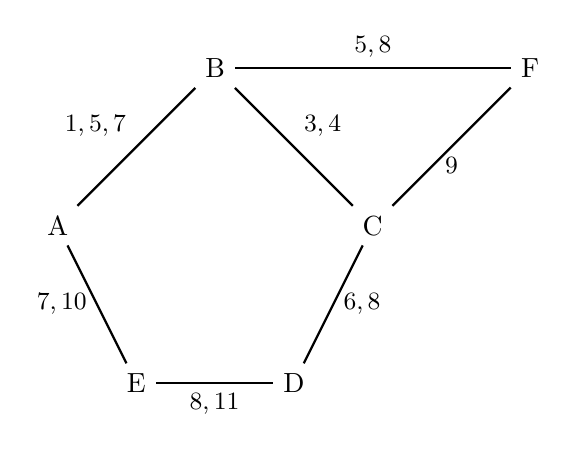
\begin{tikzpicture}[-, >=latex, node distance=2cm, thick, scale=1]
        % Nodes
        \node (A) at (0, 2) {A};
        \node (B) at (2, 4) {B};
        \node (C) at (4, 2) {C};
        \node (D) at (3, 0) {D};
        \node (E) at (1, 0) {E};
        \node (F) at (6, 4) {F};

        % Temporal edges with timestamps
        \path[every node/.style={font=\sffamily\small}]
            (A) edge node[above left] {$1,5,7$} (B)
            (B) edge node[above right] {$3,4$} (C)
            (C) edge node[right] {$6,8$} (D)
            (D) edge node[below ] {$8,11$} (E)
            (E) edge node[left] {$7,10$} (A)
            (B) edge node[above] {$5,8$} (F)
            (F) edge node[below] {$9$} (C);

        % Title
        %\node[below of=F, node distance=2cm] {Temporal Graph};
    \end{tikzpicture}
\caption{Example of a multi-labeled temporal graph. Multiple time labels are separated by commas.}
\label{fig:mulit_temporal_graph}
\end{figure}

%\begin{figure}[h!]
%\centering
%\begin{tikzpicture}[-, >=latex, node distance=2cm, thick]
%        % Nodes
%        %\node (A) at (0, 2) {A};
%        \node (B) at (2, 4) {B};
%        \node (C) at (4, 2) {C};
%        %\node (D) at (3, 0) {D};
%        %\node (E) at (1, 0) {E};
%        \node (F) at (6, 3) {F};
%
%        % Temporal edges with timestamps
%        \path[every node/.style={font=\sffamily\small}]
%            %(A) edge node[above left] {1/5/7} (B)
%            (B) edge node[above right] {4} (C)
%            %(C) edge node[right] {6/8} (D)
%            %(D) edge node[below ] {8/11} (E)
%            %(E) edge node[left] {7/10} (A)
%            (B) edge node[above] {5/8} (F)
%            (F) edge node[below] {9} (C);
%
%    \end{tikzpicture}
%\caption{Example of a multi-labeled temporal graph.}
%\label{fig:temporal_graph}
%\end{figure}

For simplicity, this article focuses on undirected temporal graphs; however, all concepts and methods can naturally extend to directed temporal graphs. When the context is clear, a temporal edge is referred to simply as an \textit{edge}. By ignoring timestamps and duplicate edges, a temporal graph induces a simple static graph, commonly referred to as the \textbf{aggregate graph} \( G \) of \( T \). In \( G \), a pair \( (u, v) \) is an edge if and only if there exists a temporal edge \( (u, v, t) \) in \( T \).\\

%\paragraph{Temporal Reachability:} One of the fundamental concepts in temporal networks is \textit{temporal reachability}. A vertex \( v \) is said to be \textbf{reachable} from another vertex \( u \) if there exists a temporal path \(\{ (u, v_1, t_1), (v_1, v_2, t_2), \ldots, (v_n, v, t_n) \} \) such that \( t_i \leq t_{i+1} \) for all \( i \in [1, n-1] \). Unlike static networks, where paths are defined by the presence of edges regardless of time, temporal reachability depends on the timing of interactions. This distinction is crucial for modeling processes that rely on the timing and sequence of interactions, such as the spread of information or diseases.


%\begin{definition} \label{def:dtg}
%A directed temporal graph $G$ consists of a finite set $V$ of nodes and a finite set $E \subseteq V \times V \times \mathbb{N} $ 
%%of ordered pairs of nodes 
%of interactions. An interaction $e \in E$
%is represented by a three-tuple $e = (u, v, t)$, in which $u$ is the source node, $v$
%is the target node and $t$ is the initiation time of the interaction.
%\end{definition}

%\begin{definition}\label{def:timerespectinginter}
%Let $e_i = (u_i, v_i, t_i)$ and $e_j = (u_j, v_j , t_j)$ be two interactions in a directed temporal graph $G$. Given some threshold $d$, the interactions are \textit{timerespecting} if they are adjacent edges and:
%
%\begin{enumerate}
%    \item $0 \leq t_j - t_i \leq d; \text{ if } v_i = u_j,$
%    \item $0 \leq t_i - t_j \leq d; \text{ if } u_i = v_j,$
%    \item $0 \leq |t_j - t_i| \leq d; \text{ otherwise}$.
%\end{enumerate} 
%\end{definition}

\paragraph{\bf{$\delta$-Temporal Motifs:}}\label{def:temporal_motif}  $\delta$-Temporal motifs, introduced in~\cite{paranjape2017motifs}, extend the concept of motifs (recurring subgraphs) from static to temporal graphs. This concept is central to our work. We recall the definition of $\delta$-temporal motifs from~\cite{paranjape2017motifs} in the context of undirected temporal graphs. A $k$-node, $l$-edge, \textbf{$\delta$-temporal motif} is a sequence of $l$ edges, $M = \{(u_1, v_1, t_1), (u_2, v_2, t_2), \dots, (u_l, v_l, t_l)\}$ such that the edges are time-ordered within a $\delta$ duration, i.e., 
\(
t_1 < t_2 < \dots < t_l \quad \text{and} \quad t_l - t_1 \leq \delta,
\)
and the induced aggregate graph from the edges is connected and has $k$ nodes.
Note that with this general definition, multiple edges between the same pair of nodes may appear in the motif \( M \). However, we restrict our attention to the case where for any pair of temporal edges \( (u_i, v_i, t_i), (u_j, v_j, t_j) \) in \( M \), it is not true that \( u_i = u_j \) and \( v_i = v_j \)\footnote{This restriction is necessary to define a filtration of simplicial complexes.}. See Figure~\ref{fig:four_motifs} for examples.

\begin{figure}[h!]
%\centering
\begin{minipage}{0.2\textwidth}
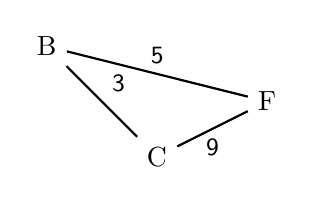
\begin{tikzpicture}[scale=0.7, -, >=latex, node distance=2cm, thick]
        % Nodes
        %\node (A) at (0, 2) {A};
        \node (B) at (2, 4) {B};
        \node (C) at (4, 2) {C};
        %\node (D) at (3, 0) {D};
        %\node (E) at (1, 0) {E};
        \node (F) at (6, 3) {F};

        % Temporal edges with timestamps
        \path[every node/.style={font=\sffamily\small}]
            %(A) edge node[above left] {1/5/7} (B)
            (B) edge node[above right] {3} (C)
            %(C) edge node[right] {6/8} (D)
            %(D) edge node[below ] {8/11} (E)
            %(E) edge node[left] {7/10} (A)
            (B) edge node[above] {5} (F)
            (F) edge node[below] {9} (C);

    \end{tikzpicture}
\end{minipage}
\hfill
\begin{minipage}{0.2\textwidth}
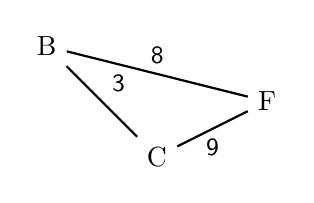
\begin{tikzpicture}[scale=0.7, -, >=latex, node distance=2cm, thick]
        % Nodes
        %\node (A) at (0, 2) {A};
        \node (B) at (2, 4) {B};
        \node (C) at (4, 2) {C};
        %\node (D) at (3, 0) {D};
        %\node (E) at (1, 0) {E};
        \node (F) at (6, 3) {F};

        % Temporal edges with timestamps
        \path[every node/.style={font=\sffamily\small}]
            %(A) edge node[above left] {1/5/7} (B)
            (B) edge node[above right] {3} (C)
            %(C) edge node[right] {6/8} (D)
            %(D) edge node[below ] {8/11} (E)
            %(E) edge node[left] {7/10} (A)
            (B) edge node[above] {8} (F)
            (F) edge node[below] {9} (C);

    \end{tikzpicture}
\end{minipage}
\hfill
\begin{minipage}{0.2\textwidth}
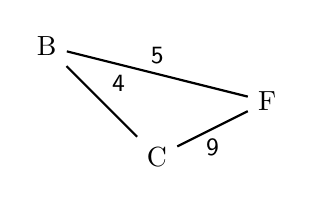
\begin{tikzpicture}[scale=0.7, -, >=latex, node distance=2cm, thick]
        % Nodes
        %\node (A) at (0, 2) {A};
        \node (B) at (2, 4) {B};
        \node (C) at (4, 2) {C};
        %\node (D) at (3, 0) {D};
        %\node (E) at (1, 0) {E};
        \node (F) at (6, 3) {F};

        % Temporal edges with timestamps
        \path[every node/.style={font=\sffamily\small}]
            %(A) edge node[above left] {1/5/7} (B)
            (B) edge node[above right] {4} (C)
            %(C) edge node[right] {6/8} (D)
            %(D) edge node[below ] {8/11} (E)
            %(E) edge node[left] {7/10} (A)
            (B) edge node[above] {5} (F)
            (F) edge node[below] {9} (C);

    \end{tikzpicture}
\end{minipage}
\hfill
\begin{minipage}{0.2\textwidth}
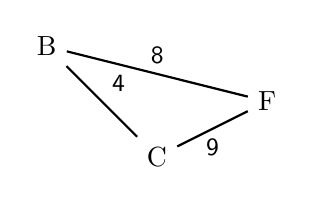
\begin{tikzpicture}[scale=0.7, -, >=latex, node distance=2cm, thick]
        % Nodes
        %\node (A) at (0, 2) {A};
        \node (B) at (2, 4) {B};
        \node (C) at (4, 2) {C};
        %\node (D) at (3, 0) {D};
        %\node (E) at (1, 0) {E};
        \node (F) at (6, 3) {F};

        % Temporal edges with timestamps
        \path[every node/.style={font=\sffamily\small}]
            %(A) edge node[above left] {1/5/7} (B)
            (B) edge node[above right] {4} (C)
            %(C) edge node[right] {6/8} (D)
            %(D) edge node[below ] {8/11} (E)
            %(E) edge node[left] {7/10} (A)
            (B) edge node[above] {8} (F)
            (F) edge node[below] {9} (C);

    \end{tikzpicture}
\end{minipage}
\caption{All four possible 3-node 3-edge motifs of Figure~\ref{fig:mulit_temporal_graph} are depicted here. Note that the temporal edges between $B$ and $C$ and $B$ and $F$ differ in their respective timestamps. The two left motifs satisfy $\delta = 6$, while the two right motifs satisfy $\delta = 5$.
}
\label{fig:four_motifs}
\end{figure}




\subsection{Topological Data Analysis}
\iffalse
In this subsection we will briefly recall the basic notions in topology that are used in TDA and then describe the standard pipeline of Persistent Homology computation. For further reading see~\cite{Hatcher2002, Edelsbrunner2010}.

A \textbf{geometric $k$-simplex} is the convex hull of $k+1$ affinely independent points in $\mathbf{R}^d$. For example, a point is a $0$-simplex, an edge is a $1$-simplex, a triangle is a $2$-simplex, and a tetrahedron is a $3$-simplex. A subset simplex is called a \textbf{face} of the original simplex. A \textbf{geometric simplicial complex} $K$ is a collection of geometric simplices that intersect only at their common faces and are closed under the \textit{face} relation. See Figure~\ref{fig:simpcompexp}
for an example. A \textbf{filtration} or a \textbf{filtered simplicial complex} $\mathcal{F}$: $\{K_1 \hookrightarrow K_2 \hookrightarrow \cdots \hookrightarrow K_m \}$ is a sequence
of nested simplicial complexes indexed by a scale parameter.\\
\textit{Homology}, is a tool from algebraic topology to quantify the number of $k$-dimensional topological features (or holes) in a topological space, such as a simplicial complex. For instance, $H_0$ the zero degree homology classes describe the number of connected components, $H_1$ the one degree homology classes describe the number of loops, and $H_2$, the two dimensional homology classes quantifies voids or cavities. The ranks of these homology groups are referred to as \textbf{Betti numbers}. In particular, the Betti number $\beta_ k$ corresponds to the number of $k$-dimensional holes. In figure~\ref{fig:simpcompexp} the Betti numbers are as follows, $\beta_0 =1, \beta_1 = 1, \text{ and } \forall k \geq 2, \beta_k = 0$. \tableref{table:bettis} shows the list of non-zero Betti numbers for all connected compact oriented 2-manifolds~\citep{SeifertThrelfall1934} along with other topological invariants such as \textit{genus} $g$ and \textit{Euler Characteristic} \(\chi = \beta_0 - \beta_1 + \beta_2 \), which in this case are related as follows \(g = \frac{\beta_1}{2} = -\frac{\chi-2}{2}\).
%Also see \tableref{table:bettis} for a list of Betti numbers of some well known topological spaces along with other related topological invariants such as \textit{genus} \(g = \frac{\beta_1}{2}\) for oriented 2-manifold and \textit{Euler Characteristics} \(\chi = \beta_0 - \beta_1 + \beta_2 - \beta_3 \cdots \).
\fi

\begin{figure}
    \begin{center}
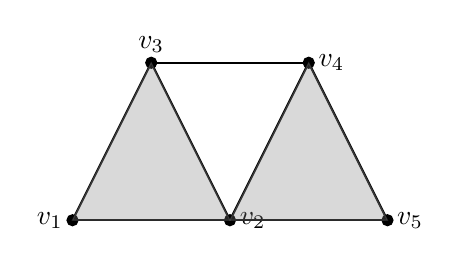
\begin{tikzpicture}

% Draw vertices
\filldraw[black] (0, 0) circle (2pt) node[anchor=east] {$v_1$};
\filldraw[black] (2, 0) circle (2pt) node[anchor=west] {$v_2$};
\filldraw[black] (1, 2) circle (2pt) node[anchor=south] {$v_3$};
\filldraw[black] (3, 2) circle (2pt) node[anchor=west] {$v_4$};
\filldraw[black] (4, 0) circle (2pt) node[anchor=west] {$v_5$};

% Draw edges
\draw[thick] (0,0) -- (2,0) node[midway, below] {};
\draw[thick] (0,0) -- (1,2) node[midway, left] {};
\draw[thick] (2,0) -- (1,2) node[midway, right] {};
\draw[thick] (2,0) -- (4,0) node[midway, below] {};
\draw[thick] (2,0) -- (3,2) node[midway, right] {};
\draw[thick] (3,2) -- (4,0) node[midway, right] {};
\draw[thick] (1,2) -- (3,2) node[midway, above] {};

% Fill in 2-simplex (triangle)
\filldraw[gray, opacity=0.3] (0,0) -- (2,0) -- (1,2) -- cycle;
\filldraw[gray, opacity=0.3] (2,0) -- (4,0) -- (3,2) -- cycle;

\end{tikzpicture}
\end{center}
    \caption{Example of a simplicial complex}
    \label{fig:simpcompexp}
\end{figure}

\iffalse

\begin{table}[ht]
\vspace{2ex}
\centering
\caption{Genus ($g$), Betti numbers ($\beta_n$), and Euler characteristic ($\chi$) of closed compact orientable surfaces.} 
\label{background:topology:table}
\begin{tabular}{lccccc}
\toprule 
Surface $M$ &$g$&$\beta_0$&$\beta_1$&$\beta_2$&$\chi$\\[3pt]\midrule
Sphere  $S^2$&0&1&0&1&2\\
Torus $T^2$&1&1&2&1&0\\
%2-holed torus $T^2 \# T^2$&2&1&4&1&-2\\
%3-holed torus $T^2  \# T^2 \# T^2$&3&1&6&1&-4\\
$g$-holed torus $T^2\# \dots \# T^2$&$g$&1&2$g$&1&2-2$g$\\[3pt]\bottomrule
\end{tabular}\label{table:bettis}
\end{table}

In a standard pipeline of \textit{persistent homology} computation, a dataset, typically represented as a point cloud in a metric space, is used to first build a filtered simplicial complex which is used to construct a \textit{boundary matrix} which is then finally reduced in a special form to read off the persistent homology. A common method for constructing such filtered simplicial complex is the \textit{Vietoris-Rips} complex. This complex is formed by connecting data points that lie within a certain distance from each other, progressively increasing the complexity of the structure as the distance threshold grows.
The idea of filtration is used to analyze data across multiple scales. As the filtration parameter (here the distance threshold) increases, new simplices are added, enabling the tracking of how topological features, such as Betti numbers, emerge and disappear across different scales. \\

\fi

\paragraph{\bf{Simplicial Complex:}}
A \textbf{geometric $k$-simplex} is the convex hull of $k+1$ affinely independent points in $\mathbf{R}^d$. For example, a point is a $0$-simplex, an edge is a $1$-simplex, a triangle is a $2$-simplex, and a tetrahedron is a $3$-simplex. A subset simplex is called a \textbf{face} of the original simplex. A \textbf{geometric simplicial complex} $K$ is a collection of geometric simplices that intersect only at their common faces and are closed under the \textit{face} relation. See Figure~\ref{fig:simpcompexp}
for an example. We will refer to a \textit{geometric simplicial complex} as simply a \textit{simplicial complex} or just a \textit{complex}.  %A simplex is called \textbf{maximal} if it is not a proper subset of any other simplex in $\textit{K}$. 
A subcollection $\textit{L}$ of $\textit{K}$ is called a \textbf{subcomplex} if it is also a simplicial complex. 
%An inclusion $\psi : K \xhookrightarrow{\sigma} K \cup \sigma$ of a single simplex $\sigma$ is called \textbf{elementary}, otherwise, it is called \textbf{non-elementary}.

A complex $K$ is a \textbf{flag} or \textbf{clique} complex if, whenever a subset of its vertices forms a clique (i.e., any pair of vertices is connected by an edge), they span a simplex. It follows that the full structure of $K$ is determined by its 1-skeleton (or graph), which we denote by $G$.

\paragraph{\bf{Homology:}} \textit{Homology} is a tool from algebraic topology to quantify the number of $k$-dimensional topological features (or holes) in a topological space, such as a simplicial complex. For instance, $H_0$ the zero degree homology class describes the number of connected components, $H_1$ the one degree homology class describes the number of loops, and $H_2$, the two dimensional homology class quantifies voids or cavities. The ranks of these homology groups are referred to as \textbf{Betti numbers}. In particular, the Betti number $\beta_ k$ corresponds to the number of $k$-dimensional holes. In Figure~\ref{fig:simpcompexp} the Betti numbers are as follows, $\beta_0 =1, \beta_1 = 1, \text{ and } \forall k \geq 2, \beta_k = 0$.

\paragraph{\bf{Filtration:}}
A \textbf{sequence} of simplicial complexes $\mathcal{F}$: $\{K_1 \hookrightarrow K_2 \hookrightarrow \cdots \hookrightarrow K_m \}$ connected through inclusion maps is called a \textbf{filtration}. A filtration is called a \textbf{flag filtration} if all the simplicial complexes $K_i$ are flag complexes. Given a weighted graph $G = (V, E, w : E \rightarrow \mathbb{R})$, a flag filtration $F_G$ can be defined by assigning the maximum weight of edges in a simplex (clique) as its filtration value. Flag filtrations are among the most common types of filtrations used in TDA applications. The concept of filtration is used to analyze data across multiple scales. As the filtration \textit{parameter} increases, new simplices are added, allowing us to track topological features, such as Betti numbers, emerge and disappear across different scales. The next paragraph formalizes this intuition.

%In a standard pipeline of \textit{persistent homology} computation, a dataset, typically represented as a point cloud in a metric space or a filtered graph, is used to first build a filtered simplicial complex which is used to construct a \textit{boundary matrix} which is then finally reduced in a special form to read off the persistent homology. 

% A common method for constructing such filtered simplicial complex is the \textit{Vietoris-Rips} complex. This complex is formed by connecting data points that lie within a certain distance from each other, progressively increasing the complexity of the structure as the distance threshold grows. 


\paragraph{\bf{Persistent Homology:}} If we compute the homology groups of all the $K_i$, we obtain the sequence $\mathcal{P}(\mathcal{F})$: $\{H_p(K_1) \xrightarrow{*} H_p(K_2) \xrightarrow{*} \cdots \xrightarrow{*} H_p(K_m)\}$. Here $H_p()$ denotes the homology group of dimension $p$ with coefficients from a field $\mathbb{F}$, and $\xrightarrow{*}$ is the homomorphism induced by the inclusion map. $\mathcal{P}(\mathcal{F})$ forms a sequence of vector spaces connected through the homomorphisms, called a \textbf{persistence module}. %More formally, a \textit{persistence module} $\mathbb{V}$ is a sequence of vector spaces $\{V_1 \rightarrow V_2 \rightarrow V_3 \rightarrow \cdots \rightarrow V_m\}$ connected by homomorphisms. A persistence module arising from a sequence of simplicial complexes captures the evolution of the topology across the sequence.

Any persistence module can be \textit{decomposed} into a collection of simpler interval modules of the form $[i, j)$~\cite{zomorodian2005computing}. The multiset of all intervals $[i, j)$ in this decomposition is called the \textbf{persistence diagram} of the persistence module. An interval of the form $[i, j)$ in the persistence diagram of $\mathcal{P}(\mathcal{F})$ corresponds to a homological feature (a ‘cycle’) that appears at $i$ and disappears at $j$. The persistence diagram (PD) completely characterizes the persistence module, providing a bijective correspondence between the PD and the equivalence class (isomorphic) of the persistence module~\cite{Edelsbrunner2010, zomorodian2005computing}. 

%The \textit{bottleneck distance} is a metric to compare two persistence diagrams \( D_1 \) and \( D_2 \), which are multisets of points \((b, d)\) representing topological features. It measures the minimum cost to match points in \( D_1 \) and \( D_2 \), allowing matches with the diagonal \( \Delta \) for unmatched points. Formally, it is defined as:

%\[
%W_{\infty}(D_1, D_2) = \inf_{\gamma} \sup_{x \in D_1} \| x - \gamma(x) \|_{\infty},
%\]

%where \( \gamma \) is a bijection between \( D_1 \cup \Delta \) and \( D_2 \cup \Delta \), and \( \| x - \gamma(x) \|_{\infty} = \max(|b_1 - b_2|, |d_1 - d_2|) \). This distance captures the maximum discrepancy between matched points and is stable under small perturbations.


\subsection{Kernel and Support Vector Machine}

%\paragraph{Kernel:}
%A \textbf{kernel} in machine learning and data analysis is a function that computes a similarity (inner product) between two data points in a potentially high-dimensional space without explicitly mapping the data to that space. % Kernels are foundational in algorithms like Support Vector Machines (SVMs), kernel PCA, and Gaussian Processes. They enable powerful transformations of data, making complex patterns more accessible for linear analysis.
%Given a set of points \( x \) and \( y \) in an input space \( X \), a \textbf{kernel} function \( \mathit{k}: X \times X \rightarrow \mathbb{R} \) is defined as: $\mathit{k}(x, y) = \langle \phi(x), \phi(y) \rangle,$ where \( \phi \) is a mapping from the input space \( X \) to a higher-dimensional feature space \( \mathcal{F} \). The function $\mathit{k}$ is \emph{symmetric} and \emph{positive semi-definite} (the corresponding Gram matrix). The kernel \( \mathit{k}(x, y) \) computes the inner product of \( \phi(x) \) and \( \phi(y) \) in \( \mathcal{F} \) without needing to explicitly compute \( \phi \), a property known as the \textit{kernel trick}. A very common kernel is the \textit{Gaussian Kernel}: \( \mathit{k}(x, y) = \exp\left(-\frac{\|x - y\|^2}{2\sigma^2}\right) \), which maps to an infinite-dimensional feature space.


\paragraph{\bf{Kernel for Persistence Diagrams:}} A kernel for persistence diagrams quantifies the similarity between diagrams by computing a weighted sum of inner products of feature points \footnote{A direct measure of distance between persistence diagrams is the \textit{bottleneck distance}~\cite{cohen2007stability}. However, since the space of persistence diagrams is non-linear, kernel-based distances are more suitable for machine learning applications.}. A commonly used kernel for PDs is the Persistence Scale Space (PSS) Kernel.  %The PSS Kernel accomplishes this by mapping persistence points to a new space where their distances are well-defined and meaningful~\cite{kusano2016persistence}. 
The \textbf{Persistence Scale Space (PSS) Kernel}~\cite{reininghaus2015stable} is defined for two persistence diagrams \( D \) and \( D' \) as follows:
\[
K_{PSS}(D, D') = \frac{1}{8\pi \sigma^2}\sum_{(p \in D)} \sum_{(q \in D')} e^{\left(-\frac{1}{8\sigma} \left( \| p - q \|^2 \right) \right)} - e^{\left(-\frac{1}{8\sigma} \left( \| p - \bar{q} \|^2 \right) \right)},
\]
where \(\sigma\) is a bandwidth parameter and $\bar{q} = (b, a)$ is $q = (a, b)$ mirrored at the diagonal. The PSS Kernel is stable under small perturbations of the input, ensuring that small changes in the diagram do not result in drastic kernel value changes, which is essential for robust applications in noisy data. The PSS Kernel enables the analysis and comparison of persistence diagrams using a continuous and differentiable kernel function, making it suitable for integration with machine learning tasks, especially in non-Euclidean data settings~\cite{reininghaus2015stable}.

\iffalse
\paragraph{\bf{Support Vector Machine (SVM):}}
A \textbf{Support Vector Machine (SVM)} is a supervised learning algorithm primarily used for classification. It aims to find the optimal hyperplane that separates different classes in a high-dimensional space. Given a training dataset \( \{(\mathbf{x}_i, y_i)\}_{i=1}^n \), where \( \mathbf{x}_i \in \mathbb{R}^d \) and \( y_i \in \{-1, 1\} \), SVM solves the optimization problem:
 $\min_{\mathbf{w}, b} \frac{1}{2} \|\mathbf{w}\|^2,$
subject to: $y_i (\mathbf{w} \cdot \mathbf{x}_i + b) \geq 1, \quad \forall i.$ SVM aims to maximize the margin between classes, ensuring robust classification even with overlapping data points.
\fi

\iffalse
\section{Topological Data Analysis (TDA)}

Topological Data Analysis (TDA) is an emerging field that utilizes concepts from topology to analyze the shape of data, offering a unique way to study high-dimensional and complex datasets. One of the most widely used tools in TDA is \textit{persistent homology}, which measures topological features such as connected components, loops, and voids across multiple scales. The persistent nature of these features makes TDA robust against noise and small perturbations in data.

TDA has found significant success across various domains. In \textbf{biology}, TDA has been used to analyze gene expression data and to identify meaningful structures within high-dimensional biological datasets. For example, it has been applied in the study of cancer types, revealing new subtypes and relationships among gene expression patterns that were previously undetected \cite{nicolau2011topology}. Similarly, in neuroscience, TDA has been employed to study brain connectivity, helping researchers understand how neural activities shape learning and memory \cite{sizemore2019importance}.

In the field of \textbf{machine learning}, TDA enhances traditional algorithms by introducing shape-based features. TDA has been successfully used in image recognition, classification, and clustering tasks. One prominent example is its application to improve deep learning models by integrating topological features with neural network architectures, which has been shown to boost accuracy and robustness \cite{hofer2017deep}.

Moreover, in \textbf{sensor networks} and \textbf{geospatial analysis}, TDA has been instrumental in identifying coverage holes and optimizing network layouts. TDA methods have been utilized to assess the structure and stability of networks over time and to determine important regions within sensor arrays or geographic regions \cite{adams2017persistence}. For example, TDA has been used to model and analyze the temporal changes in urban traffic networks to improve traffic management and planning \cite{ghrist2008barcodes}.

The application of TDA in \textbf{finance} is another success story, where it has been applied to identify patterns in market behavior. In particular, TDA has helped in modeling the structure of stock market data, providing insights into market stability, the formation of bubbles, and risk assessment by analyzing the evolving topology of financial networks \cite{gidea2018topological}.

These examples highlight the versatility of TDA in handling complex, noisy, and high-dimensional data across different domains. Its ability to reveal intrinsic data structures and provide novel insights makes it a powerful tool for modern data science.


\section{Temporal Graph}

We refer an “edge” between two nodes, as “interaction” to emphasize the encoded time as part of the network representation. An interaction is specified as a triplet, made up of two nodes and the time of their contact.


\begin{definition} \label{def:dtg}
A directed temporal graph $G$ consists of a finite set $V$ of nodes and a finite set $E \subseteq V \times V \times \mathbb{N} $ 
%of ordered pairs of nodes 
of interactions. An interaction $e \in E$
is represented by a three-tuple $e = (u, v, t)$, in which $u$ is the source node, $v$
is the target node and $t$ is the initiation time of the interaction.
\end{definition}

We say that a temporal graph $T = (V,E)$ is single labelled temporal graph if for every tuple $(u,v) \in V \times V$, 
there is at most one interaction of the form $(u,v,t)$ or $(v,u,t) \in E$.
In a directed temporal network, we have the notion of a contagion being
initiated by an individual and spreading over a sequence of interactions to others
in the network. In order for a contagion to take place, adjacent interactions must
be time-respecting.

\begin{definition}\label{def:timerespectinginter}
Let $e_i = (u_i, v_i, t_i)$ and $e_j = (u_j, v_j , t_j)$ be two interactions in a directed temporal graph $G$. Given some threshold $d$, the interactions are \textit{timerespecting} if they are adjacent edges and:

\begin{enumerate}
    \item $0 \leq t_j - t_i \leq d; \text{ if } v_i = u_j,$
    \item $0 \leq t_i - t_j \leq d; \text{ if } u_i = v_j,$
    \item $0 \leq |t_j - t_i| \leq d; \text{ otherwise}$.
\end{enumerate} 
\end{definition}

% \ref{def:timerespectinginter}

In the first two cases of Definition (put reference), The interactions meet head-to-tail. In the third case, the interactions either share a source node or a target node. This relation between time-respecting interactions is a constraint, which we
incorporate into our definition of a time-respecting path and subgraph.

%Time-respecting paths describe a non-decreasing sequence of interactions cite[(Pan & Saram¨aki, 2011)]. A path can be thought of as a mechanism for passing information from a source, along a sequence of intermediaries, to a target. This serves to emphasize our view of the network from a temporal standpoint. With traditional time-slicing, the specified time window determines which interactions are examined, between a minimum and maximum interaction time. However, a time-respecting path has no such bounds. In fact, given the right connectivity and timing of interactions, a path might be initiated when the network is first created, and continue until the latest point in the data set.

We define a time-respecting subgraph in terms of time-respecting interactions. 
\begin{definition} Given a real parameter $d \geq 0$, a time-respecting subgraph $G_d = (V', E')$  of a temporal graph
$T = (V, E)$ is a subgraph such that every adjacent interaction pair in $E'$ is
time-respecting with respect to $d$.
\end{definition}

Using the notion of time-respecting subgraphs we define weights on the edges of the temporal graph $G$, which is in turn used to define filtration on the clique complex $cl(G)$ of $G$.
\begin{definition}\label{def:filt1} Let $e = (u,v,t)$ be an interaction in a temporal $T = (V, E)$, the weight of $e$ is the smallest $d \geq 0$ such that there exists a time respecting subgraph $G_d = (V', E')$ for parameter $d$.    
\end{definition}

As explained above, this defines a weight function on a temporal graph and that in turn gives us way to define filtration on the clique complex of the graph. 
Defining such weight function enables us to use plethora of already developed techniques to analyse the temporal graphs including kernel methods etc. Moreover, the computation of these edges weights can be done very efficiently.
Next we describe algorithms and data-structure to compute the weight function. 


\begin{definition}
    \label{sparcity}
    Let $T = (V,E)$ be a temporal graph. We define the sparcity of $G$ to be 
    $\frac{2|\tilde{E}|}{|V|^2}$ where $\tilde{E} = \{ (u,v) \mid (u,v,t) \in E \}$ for some $ t \in \mathbb{N}$.
\end{definition}




\subsection{Data-Structure}
A standard data structure such as adjacency list or adjacency matrix for a directed graph can easily be adapted to store the temporal information associated with the edges. WE CAN EXPAND THIS SECTION LATER.

\fi

\section{Temporal Filtrations}\label{sec:temp_filtration}
In this section, we introduce a simple method and an algorithm for constructing filtered (weighted) graphs from single-labeled, and multi-labeled temporal graphs. The filtered graph captures the evolution of fixed-size (\(3\)-node, \(2\)-edge) \( \delta \)-temporal motifs. %for increasing values of \( \delta > 0 \) in the given temporal graph. %The corresponding persistence diagram, computed by treating the filtered graph as the \(1\)-skeleton of a flag filtration, effectively captures the global `temporal topology' of the temporal graph. These diagrams are powerful tools for analyzing temporal graphs. In Section~\ref{sec:experiments}, we employ these diagrams for classifying temporal graphs.


\subsection{Single Labeled Temporal Graphs}\label{single_filtration}
\paragraph{\bf{The Average Filtration:}}
Let \( T = (V, E) \) be a single-labeled temporal graph, we construct a filtered simple graph \( G_f = (V_f, E_f, f_\mathrm{avg}: (V_f \cup E_f) \to \mathbb{R}) \) derived from \( T \).  The vertex set \( V_f \) of \( G_f \) is identical to \( V \), and the edge set \( E_f \) of \( G_f \) corresponds to the edges in the aggregate graph \( G \) of \( T \). Specifically, for each temporal edge \( (u, v, t) \in E \) in \( T \), there exists a corresponding edge \( (u, v) \in E_f \) in \( G_f \). Notably, \( G_f \) is a simple graph, meaning that no multiple edges exist between any pair of vertices. The filtration \( f_\mathrm{avg}: (V_f \cup E_f) \to \mathbb{R} \) is referred to as the \textbf{average filtration}.

To motivate the definition of the average filtration \( f_\mathrm{avg} \), we first introduce the concept of the \textbf{minimum filtration} \( f_\mathrm{min}: (V_f \cup E_f) \to \mathbb{R} \). We begin by assigning a filtration value of \( 0 \) to all vertices in \( V_f \), i.e., \( f_\mathrm{avg}(V_f) = 0 \). We then describe the method for computing the filtration values of the edges in \( G_f \).

Let \( \nedges(u,v) := \{ (u', v', t) \mid u = u' \text{ or } v = v' \} \setminus \{ (u, v, t) \} \) represent the set of adjacent temporal edges of \( (u, v, t) \) in \( T \), where each interaction \( (u, v, t) \) belongs to \( T \). Additionally, let \( \tim(u, v) := t \) denote the time label of the edge \( (u, v) \) in \( T \).
%Note that $\tim$ is well defined since $G$ is a single labeled temporal graph.
The filtration value of each edge \( (u,v) \) in \( G_f \) is computed using the minimum of the difference in time stamps between the edge \( (u,v) \) and its adjacent interactions in \( T \):
$$ f_\mathrm{min}(e) := \min_{e' \in \nedges(e)} | \tim(e) - \tim(e')|.$$

As previously mentioned, we aim to capture the evolution of \(\delta\)-temporal motifs within a temporal graph through temporal filtrations. By fixing the values of \(k\) (number of nodes) and \(l\) (number of edges), one can canonically define a filtration over the temporal graph by varying the parameter \(\delta\). Specifically, for each edge \((u, v)\) in a temporal graph, its filtration value is assigned as the smallest \(\delta\) for which it belongs to a fixed $k$ and $l$ \(\delta\)-temporal motif. For \(k = 3\) and \(l = 2\), this canonical filtration corresponds to the minimum filtration \(f_\mathrm{min}\), as defined above.


The minimum filtration \(f_\mathrm{min}\) is highly sensitive to changes in interactions, particularly those corresponding to the minimum value, and it often fails to robustly capture the relational and global `temporal connectivity' of the graph. To address this limitation, we redefine the filtration value of an edge as the average of all \(\delta\)-values in the smallest (w.r.t to the parameter $\delta$) \(\delta\)-temporal motifs that include the edge. Specifically, the \textit{average filtration} of the edges in \(G_f\) is defined as:

$$ f_\mathrm{avg}(e) := \frac{\sum_{e' \in \nedges(e)} | \tim(e) - \tim(e')|}{|\nedges(e)|}.  $$


%\sid{Question: How would a temporal graph of one edge would work? We should also discuss what would a maximum filtration do.}
The average filtration reflects the relative temporal importance of an edge: a smaller filtration value indicates that more and faster temporal paths pass through the edge.
 
The examples in Figure~\ref{fig:avg_min_filt} illustrate the distinction between the average and minimum filtrations. The temporal loop \(ABCDEA\) in the original temporal graph (left of Figure~\ref{fig:avg_min_filt}) has a temporal length of 9 and can be constructed from smaller \(\delta\)-temporal motifs with 3 nodes and 2 edges for \(\delta = 9\). However, in the minimum filtration, the cycle appears at \(\delta = 2\), while in the average filtration, it emerges at \(\delta = 5.5\). Additionally, the average filtration produces more widely distributed filtration values. This difference suggests that the average filtration takes into account a broader neighborhood around each edge, assigning values that more accurately reflect the relative `temporal position' of the edges. This characteristic makes the average filtration more stable and discriminative compared to the minimum filtration. Experimental results further validate this observation.


\begin{figure}[h!]
\begin{minipage}{0.3\textwidth}
\centering
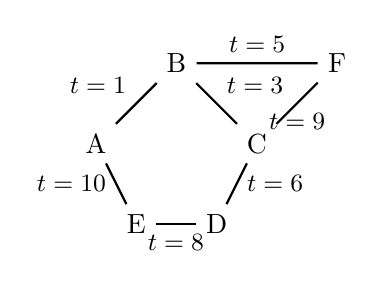
\begin{tikzpicture}[scale = 0.6, -, >=latex, node distance=2cm, thick,scale=0.85]
        % Nodes
        \node (A) at (0, 2) {A};
        \node (B) at (2, 4) {B};
        \node (C) at (4, 2) {C};
        \node (D) at (3, 0) {D};
        \node (E) at (1, 0) {E};
        \node (F) at (6, 4) {F};

        % Temporal edges with timestamps
        \path[every node/.style={font=\sffamily\small}]
            (A) edge node[above left] {$t=1$} (B)
            (B) edge node[above right] {$t=3$} (C)
            (C) edge node[right] {$t=6$} (D)
            (D) edge node[below] {$t=8$} (E)
            (E) edge node[left] {$t=10$} (A)
            (B) edge node[above] {$t=5$} (F)
            (F) edge node[below] {$t=9$} (C);

        % Title
        %\node[below of=F, node distance=2cm] {Temporal Graph};
    \end{tikzpicture}
%\caption{A single-labeled temporal graph.}
\label{fig:single_temporal_graph}
\end{minipage}
\hfill
\begin{minipage}{0.3\textwidth}
    \centering
    % Graph with Average Filtration Labels
    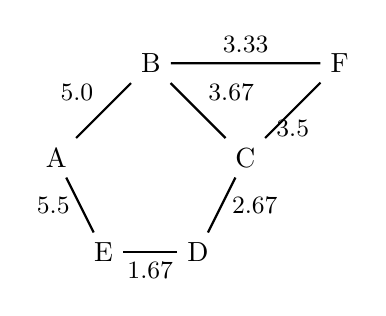
\begin{tikzpicture}[scale = 0.6, -, >=latex, node distance=2cm, thick,scale=1]
        % Nodes
        \node (A) at (0, 2) {A};
        \node (B) at (2, 4) {B};
        \node (C) at (4, 2) {C};
        \node (D) at (3, 0) {D};
        \node (E) at (1, 0) {E};
        \node (F) at (6, 4) {F};

        % Edges with Average Filtration Values
        \path[every node/.style={font=\sffamily\small}]
            (A) edge node[above left] {$5.0$} (B)
            (B) edge node[above right] {$3.67$} (C)
            (C) edge node[right] {$2.67$} (D)
            (D) edge node[below] {$1.67$} (E)
            (E) edge node[left] {$5.5$} (A)
            (B) edge node[above] {$3.33$} (F)
            (F) edge node[below] {$3.5$} (C);

        % Title
        %\node[below of=F, node distance=2cm] {Graph with Average Filtration Labels};
    \end{tikzpicture}
\end{minipage} 
\hfill
\begin{minipage}{0.3\textwidth}
    \centering
    % Graph with Min Filtration Labels
    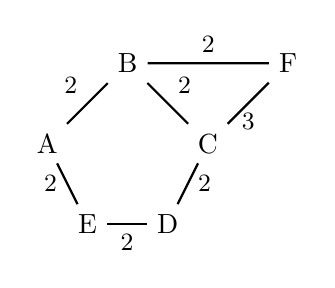
\begin{tikzpicture}[scale = 0.6,-, >=latex, node distance=2cm, thick, scale=0.85]
        % Nodes
        \node (A) at (0, 2) {A};
        \node (B) at (2, 4) {B};
        \node (C) at (4, 2) {C};
        \node (D) at (3, 0) {D};
        \node (E) at (1, 0) {E};
        \node (F) at (6, 4) {F};

        % Edges with Min Filtration Values
        \path[every node/.style={font=\sffamily\small}]
            (A) edge node[above left] {$2$} (B)
            (B) edge node[above right] {$2$} (C)
            (C) edge node[right] {$2$} (D)
            (D) edge node[below] {$2$} (E)
            (E) edge node[left] {$2$} (A)
            (B) edge node[above] {$2$} (F)
            (F) edge node[below] {$3$} (C);

        % Title
        %\node[below of=F, node distance=2cm] {Graph with Min Filtration Labels};
    \end{tikzpicture}
    \end{minipage}
        \caption{The first figure on the left shows a single-labeled temporal graph, followed by the corresponding average and minimum filtrations derived from it in the next two figures.
}\label{fig:avg_min_filt}
\end{figure}
 
We fix the size of the \( \delta \)-temporal motifs to be \( 3 \)-node, \( 2 \)-edge, as it is the smallest (and perhaps only) motif that captures the complete global connectivity of the temporal graph. The example in Figure~\ref{fig:four_motifs} clearly illustrates this; all possible \( 3 \)-node, \( 3 \)-edge \( \delta \)-temporal motifs in the figure would fail to cover the entire temporal graph.

\paragraph{Algorithm: }
We present an efficient algorithm for computing the average filtration of a temporal graph \( T = (V, E) \). The main idea of the algorithm is as follows: we first iterate over the vertices \( V \) of the graph. For each vertex \( v \in V \), we examine the set of edges \( E_v \subset E \) incident to \( v \). Any two such incident edges \( e \) and \( e' \) will be adjacent and will contribute to each other's filtration values. Specifically, for each pair of incident edges, we compute the timestamp difference \( |t - t'| \), where \( t \) and \( t' \) are the respective timestamps of \( e \) and \( e' \).

To efficiently track these contributions, we maintain a sum variable \( \mathsf{S}_e \) for each edge \( e \). After calculating \( |t - t'| \), we update the sum variables for both edges as follows:
\(
\mathsf{S}_e \gets \mathsf{S}_e + |t - t'| \quad \text{and} \quad \mathsf{S}_{e'} \gets \mathsf{S}_{e'} + |t - t'|.
\)
This process is repeated for all possible pairs of incident edges on \( v \), and the vertex \( v \) is then marked as visited. Once both boundary vertices of an edge \( e = uv \) are marked as visited, we compute its filtration value:
\(
f_\mathrm{avg}(e) = \frac{\mathsf{S}_e}{td_u + td_v},
\)
where \( td_u \) and \( td_v \) are the temporal degrees of the vertices \( u \) and \( v \), respectively. See the pseudocode (Algorithm~\ref{alg:avg_filt}) for more details.


%To optimize the computation of incident temporal edges at each vertex, we store the graph as an adjacency link list of edges incident to each vertex \( v \). This makes the computation of $E_v$ in constant $\mathcal{O}(1)$ time. For each vertex we need to compare $\mathcal{O}(d_{max}^2)$ pair of incident edges, where $d_{max}$ is the maximum temporal degree of the graph. Which results in \( \mathcal{O}(|V| \times d_{max}^2) = \mathcal{O}(|E| \times d_max}\), time complexity.

To optimize the computation of incident temporal edges at each vertex, the graph is stored as an adjacency linked list of edges incident to each vertex \( v \). This representation allows the retrieval of \( E_v \) in constant \( \mathcal{O}(1) \) time. For each vertex, we compare \( \mathcal{O}(d_{\text{max}}^2) \) pairs of incident edges, where \( d_{\text{max}} \) is the maximum temporal degree of the graph. Consequently, the overall time complexity of the algorithm is: \(
\mathcal{O}(|V| \times d_{\text{max}}^2) = \mathcal{O}(|E| \times d_{\text{max}}),
\) where \( |V| \) is the total number of vertices and  \( |E| \) is the total number of temporal edges in the graph.


%To compute the average filtration, we iterate over each edge and calculate its filtration value by traversing its edge neighborhood. The overall time complexity of the algorithm is \( \mathcal{O}(|E| \times d_{max}) \), where \( |E| \) is the total number of temporal edges in the temporal graph \( T = (V, E) \). The following pseudocode provides further details of the implementation.

\begin{algorithm}
\caption{ComputeAverageFiltration }\label{alg:avg_filt}
\begin{algorithmic}[1]
%\Require Temporal graph \( T = (V, E) \), where \( E = \{(u, v, t)\} \)
%\Ensure Filtration values \( f_\mathrm{avg}(e) \) for each edge \( e \in E \)

\State Initialize \( \mathsf{S}_e \gets 0 \) for each \( e \in E \) and \( \mathsf{visited}_v \gets \text{False} \) for each \( v \in V \)
%\State Initialize \( \mathsf{visited}_v \gets \text{False} \) for each \( v \in V \)
\State Initialize an empty filtration value map \( f_\mathrm{avg} \)

\For{each vertex \( v \in V \)}
%    \If{\( \mathsf{visited}_v = \text{True} \)}
%        \State \textbf{continue}
%    \EndIf

    \State Retrieve all incident edges \( E_v = \{e = (v, u, t)\} \)
    \State Initialize a stack \( \mathsf{stack} \) with all edges \( e \in E_v \)
    
    \While{\( \mathsf{stack} \text{ is not empty} \)}
        \State Pop an edge \( e = (v, u, t) \) from \( \mathsf{stack} \)
        \For{each remaining edge \( e' = (v, w, t') \) in \( \mathsf{stack} \)}
            \State Compute \( \Delta \gets |t - t'| \)
            \State Update \( \mathsf{S}_e \gets \mathsf{S}_e + \Delta \)
            \State Update \( \mathsf{S}_{e'} \gets \mathsf{S}_{e'} + \Delta \)
        \EndFor
        
        \If{\( \mathsf{visited}_u = \text{True} \)} \Comment{ $v$ being visited is not required}
            \State Compute \( f_\mathrm{avg}(e) \gets \frac{\mathsf{S}_e}{td_v + td_u} \)
        \EndIf
    \EndWhile
    
    \State Mark \( \mathsf{visited}_v \gets \text{True} \)
\EndFor

\State \Return \( f_\mathrm{avg}(e) \) for all \( e \in E \)

\end{algorithmic}
\end{algorithm}

%Now to compute the average filtration we iterate over each edge and 
%\begin{itemize}
%    \item For each $e_i = (u_i,v_i,t_i) \in T = (V, E)$
%     \begin{enumerate}
%        \item $wt(e_i) = 0$
%        \item $ngh(e_i) = 0$
%        \item For each adjacent edge $e_j$ of $e_i$
%        \begin{enumerate}
%            \item $wt(e_i) = wt(e_i) + |t_j - t_i|$ 
%            \item $ngh(e_i) = ngh(e_i) + 1$ 
%        \end{enumerate}
%        \item if $ngh(e_i) > 0$ then $wt(e_i) = \frac{wt(e_i)}{ngh(e_i}$
%    \end{enumerate}
%    \item EndFor
%\end{itemize}

%\textbf{Complexity :} Should be $O(|E|*k)$, where $|E|$ is the total number of edges and $k$ the degree of the graph.
%
%\textbf{Proof of correctness :} For each edge the smallest time respecting subgraph must contain its neighbours as all time respecting subgraphs are connected. 

\subsection{Multi-labeled Temporal Graphs}
We now extend the average filtration of single-labeled temporal graphs to multi-labeled temporal graphs. %The main challenge arises when the filtered graph becomes non-simple, due to multiple interactions between two nodes at different timestamps. The clique complex of such a graph is not strictly simplicial, complicating the persistence diagram computation. To address this
Our approach for multi-labeled graphs follows a similar methodology as the single-labeled case. In this context, we average the time differences across multiple interactions and assign a single edge to represent the interactions.

Given a multi-labeled temporal graph \( T = (V, E) \), we construct a filtered simple graph \( G_f = (V_f, E_f, f_\mathrm{avg}^\mathrm{mlt}: (V_f \cup E_f) \to \mathbb{R}) \) derived from \( T \). Similar to the single-labeled case, the vertex set \( V_f \) and the edge set \( E_f \) of \( G_f \) correspond to the vertices and edges in the aggregate graph \( G \) of \( T \). Here, \( \tim(u,v) = \{ t \mid (u,v,t) \in E\} \) represents the set of all time labels associated with the edge \( (u,v) \). As in the single-labeled case, the filtration value of vertices is set to 0. The filtration value of the edges in \( G_f \) is computed as follows:

$$
f_\mathrm{avg}^\mathrm{mlt}(e) = \frac{\sum_{e' \in \nedges(e)} \sum_{t \in \tim(e), t' \in \tim(e')} | t - t'|}{|\nedges(e)|}.
$$


%\sid{Why not average over all the interactions rather than the number of  edges (pair of nodes).}

%Here too the filtration value of an edge corresponds to the average of all \(\delta\)-values of the smallest (w.r.t to the parameter $\delta$) \(\delta\)-temporal motifs that include the edge. 

%In the second approach, we compute the average of the time labels for interactions between a pair of nodes and assign this average as a single time label. This converts the multi-labeled temporal graph \( T \) into a single-labeled temporal graph \( T_s \). The vertices of \( T_s \) are the same as those in \( T \), and for each edge \( e \), we define the time label in \( T_s \) as:

%\[\tim_{s}(e) = \frac{\sum_{t \in \tim(e)} t}{|\tim(e)|}.\]

%Here, \( \tim_{s}(e) \) is the unique time stamp for each temporal edge in \( T_s \). The single-labeled graph \( T_s \) is then used to compute the average filtration.



%Now we convert $G_S$ to a weighted graph as described in Section~\ref{single_filtration} to compute the filtration.
%
%
%Once we create the persistence diagrams for each graph, they are stored in a text file separated by newlines. 
%The file is now parsed through a C++ program that calculates the Persistence Scale Space Kernel (cite reninghaus), which is stored in a csv.
%
%The kernel matrix is then split into train and test sub matrices according to the graphs split in train and test sets previously. 
%The precomputed kernel matrix for the train set is now fitted to a vanilla SVM classifier, and then the accuracy is tested on the test submatrix.

\section{Stability}\label{sec:Stability}

In this section, we examine the stability of the temporal filtrations defined earlier in the context of \textit{randomized reference models} of temporal graphs. To provide a foundation, we first briefly review the concept of randomized reference models and introduce some commonly used models, as outlined in \cite{Holme2012, Karsai2011}. These models form the basis for defining the various classification classes used in our experiments.

\subsection{Randomized Reference Model}
The \textit{configuration model} is a randomized reference model, commonly used in the study of static networks to compare the empirical network's features (such as clustering, path length, or other topological characteristics) with those of a randomized network. The configuration model is created by randomly shuffling the edges of a given graph while preserving some of its structural properties, most notably the degree distribution.

%For static networks, the significance or anomaly of topological features is often assessed by comparing them to a randomized reference model, such as the configuration model, which preserves the original degree sequence while randomizing links. This allows for evaluating the significance of graph characteristics through direct comparisons, statistical test scores, or differences in process dynamics between the empirical network and the reference

For temporal graphs, a similar approach involves randomizing or reshuffling event sequences (interactions) to remove time-domain structures and correlations. Unlike static networks, temporal graphs exhibit diverse temporal correlations (structures) across varying scales, making it challenging to design a single, universal null model. Karsai et.al.~\cite{Karsai2011} identify five of these temporal correlations, namely: community structure (C), weight-topology correlations (W), bursty event dynamics on single links (B), and event-event correlations between links (E) and a daily pattern (D). They also provide tailored null models that selectively remove specific correlations to analyze their influence on the observed temporal features or dynamical processes like spreading. %By comparing dynamics across models, the role of different temporal and topological correlations can be assessed.
Below, we recall three temporal null models from Karsai et al.~\cite{Karsai2011} and Holme~\cite{Holme2012}. 
 
\begin{itemize}
    \item \textbf{Equal-Weight Link-Sequence Shuffle (EWLSS):}  
    In this method, two interaction pairs \((u_1, v_1), (u_2, v_2) \in V \times V\) are randomly selected such that \(|\tim(u_1, v_1)| = |\tim(u_2, v_2)|\). Then the time labels of these selected pairs \((u_1, v_1)\) and \((u_2, v_2)\) are swapped. Note that, \(\tim(u, v)\) represents the set of time labels associated with the pair \((u, v)\). This process can be repeated multiple times to construct a new randomized temporal graph. %This process erases the previous temporal correlations between edges but retains the event counts. %For links with large weights, events are grouped into bins with 2–3 weight values to simplify the shuffling process.
	\item \textbf{Randomized Edges (RE):} Algorithmically this method could be described as follows: iterate over all edges and for each edge $(u,v)$, select another edge $(u', v')$.  With 50\% probability, replace $(u,v)$ and $(u', v')$ with $(u, v')$ and $(u', v)$; otherwise, replace them with $(u, u')$ and $(v, v')$. The times of contact for each edge remain constant and we further make sure that there are no self loops or multiple edges. %This method extends the configuration model for static graphs by preserving edge-specific contact sequences during rewiring.
 %\item \textbf{DCB (Link-Sequence Shuffled):}  Whole single-link event sequences are randomly exchanged between randomly chosen links, without considering event counts. This method eliminates both event-event correlations and weight-topology correlations.

    %\item \textbf{DCW (Time-Shuffled):}  The time stamps of all events in the original sequence are shuffled randomly. This destroys temporal correlations while preserving the overall distribution of events.

    \item \textbf{Configuration Model (CM):}  
    The aggregated graph of the temporal graph is rewired using the configuration model of the static graph, which preserves the degree distribution and overall connectivity of nodes while removing topological correlations. Then the original single-edge interaction time labels are randomly assigned to the edge, followed by time shuffling. This method destroys all correlations except broad seasonal patterns, such as daily cycles.
\end{itemize}

In addition to these three model we introduce a new null model that is suitable for some of our specific experiments.

\begin{itemize}
\item \textbf{Time Perturbation (TP):} In this method, a fraction of interactions \( e = (u, v, t) \in E \) in the original temporal graph is replaced with \( e' = (u, v, t') \), where \( |t - t'| < \epsilon \) for some \( \epsilon > 0 \). This procedure only perturbs the time stamps of the edges, preserving most of the temporal and structural features of the original temporal graph.
\end{itemize}


%This null model isolates the effect of network topology while preserving temporal correlations and edge-specific patterns like `burstiness' and inter-contact time distributions. It assumes edges govern contact times, meaning vertex contact timings and counts may vary post-randomization, but vertex degrees in the aggregated network remain unchanged. Additionally, the overall event rate over time is preserved. An illustration of this process can be found in Fig.~12.

The first model, EWLSS, preserves the daily pattern (D), the community structure (C), weight-topology correlations (W), and bursty event dynamics on individual edges (B). In contrast, the configuration model loses all temporal correlations (structures) except for the daily pattern (D). This distinction has been experimentally verified by Karsai et al.~\cite{Karsai2011}, where graphs generated using EWLSS procedures exhibit spreading dynamics closely resembling those of the original graph. On the other hand, graphs generated using the configuration model deviate significantly from the original dynamics.

We leverage these models to define and populate distinct classes for classification tasks. The configuration model generates temporal graphs with diverse dynamics, while the other three models (EWLSS, RE and TP) are used to produce graphs with similar dynamics, forming a single class. The similarity within each class depends on the model used; TP and EWLSS create more homogeneous classes compared to the RE model. Originally designed for studying spreading dynamics with the SI model~\cite{kermack1927mathematical}, these null models eliminate the need for direct SI simulations, enhancing both the efficiency and flexibility of our method without requiring labeled nodes.


\subsection{Stability} 
We now discuss the stability of our temporal filtration with respect to the above null models. In particular, we calculate the difference in the average filtrations values of the edges that are , shuffled, swapped or changed during each step of the above reference modes.\\

\subparagraph*{\textbf{TP Procedure :}}

%Given a temporal graph $T = (V, E)$, a new temporal graph is constructed by randomly perturbing a percentage of the interactions in $G$.  That is, for some $\epsilon > 0$, we replace of percentage of interactions $e = (u,v,t) \in E$ with $e' = (u , v, t')$ such that $| t - t'| < \epsilon $. This procedure only perturbs the time stamps of the edges and preserves the structure of the temporal graph. 

Let $T$ be a single-labeled temporal graph and $e = (u,v,t)$ is an interaction in $T$. Suppose the time label \( \tim(e) = t \) is replaced by \( t + \epsilon \).  The change in \( f_\mathrm{avg}(e) \), denoted by \( \Delta f_\mathrm{avg}(e) \), can be upper bounded as follows:


%Let \( f_\mathrm{avg}(e) \) denote the single-label average filtration of an edge \( e \), given by
%\[f_\mathrm{avg}(e) := \frac{\sum_{e' \in \nedges(e)} | \tim(e) - \tim(e')|}{|\nedges(e)|}.\]

\begin{align*}
    \Delta f_\mathrm{avg}(e) & = f_\mathrm{avg}(e)_{\text{new}} - f_\mathrm{avg}(e)_{\text{old}} \\ 
    & = \frac{1}{|\nedges(e)|} \sum_{e' \in \nedges(e)} \Big( |(t + \epsilon) - \tim(e')| - |t - \tim(e')| \Big).
\end{align*}

% $$
% \Delta f_\mathrm{avg}(e) = f_\mathrm{avg}(e)_{\text{new}} - f_\mathrm{avg}(e)_{\text{old}} = \frac{1}{|\nedges(e)|} \sum_{e' \in \nedges(e)} \Big( |(t + \epsilon) - \tim(e')| - |t - \tim(e')| \Big).
% $$

Let \( \tim(e') = t' \), then for each \( e' \in \nedges(e) \) the inner term is
$
| (t + \epsilon) - t'| - |t - t'| \leq \epsilon.
$
%This follows from the triangle inequality, which ensures that the change in absolute difference is bounded by \( |\epsilon| \), the shift in \( t \). Similarly:
%\[
%| (t + \epsilon) - t'| - |t - t'| \geq -\epsilon.
%\]
%
%Thus, the term \( |(t + \epsilon) - t'| - |t - t'| \) satisfies:
%\[
%-\epsilon \leq |(t + \epsilon) - t'| - |t - t'| \leq \epsilon.
%\]
%
%Summing Over Edges
%The sum \( \sum_{e' \in \nedges(e)} \) aggregates contributions from all edges \( e' \in \nedges(e) \). With \( |\nedges(e)| \) total edges, the cumulative change is bounded by:
%\[
%\sum_{e' \in \nedges(e)} \Big( |(t + \epsilon) - \tim(e')| - |t - \tim(e')| \Big) \leq \epsilon \cdot |\nedges(e)|.
%\]
%
% Final Bound
%Dividing by \( |\nedges(e)| \) to compute the average, 
we therefore obtain:
$
|\Delta f_\mathrm{avg}(e)| \leq \epsilon.
$ The filtration values of edges in the neighborhood of \( e \) also change. Using a similar computation and the fact that $\tim(e'')$ does not change for all $e'' \in \nedges(e') \setminus \{e\}$, for each \( e' \in \nedges(e) \), we can express the change as:

\begin{align*}
    \Delta f_\mathrm{avg}(e') & 
= \frac{1}{|\nedges(e')|} (|(t + \epsilon) -  \tim(e')| - |t -  \tim(e')|) = \frac{\epsilon}{|\nedges(e')|} \leq \epsilon.
\end{align*}

% Hence, 
% \(
% |\Delta f_\mathrm{avg}(e')| = \frac{\epsilon}{|\nedges(e')|} \leq \frac{\epsilon}{d_{max}},
% \)
% where \( d_{max} > 1 \) represents the maximum degree of the graph \( T \).

We use the \( L_{\infty} \) norm to measure the distance between filtrations~\cite{cohen2007stability}. The overall distance between the new (shifted) and the original average filtration of the temporal graph \( G \) is bounded above as follows:
\(
|\Delta_{\infty} f_\mathrm{avg}(G)| \leq \epsilon.
\)
Note that this bound holds even after time stamp shifts of multiple edges.


%$$  | f_\mathrm{avg}(e) - f'_{avg} (e') | = $$ 
%$$ = \frac{| \sum_{e^n \in \nedges(e)} \sum_{t_G \in \tim(e) , t^n_G \in \tim(e^n)}| t_G - t^n_G| - \sum_{e^n \in \nedges(e')} \sum_{t'_{G'} \in \tim'(e') , t^n_{G'} \in \tim'(e^n)}| t'_{G'} - t^n_{G'}| |}{|\nedges(e)|} $$
%$$ =  \frac{| \sum_{e^n \in \nedges(e)} \sum_{t_G \in \tim(e) , t'_G \in \tim(e')}| t_G - t'_G| -  \sum_{t_{G'} \in \tim' (e) , t'_{G'} \in \tim'(e')}| t_{G'} - t'_{G'}| |}{|\nedges(e)|}$$
%$$ \leq \frac{\sum_{e' \in \nedges(e)} 2 \epsilon }{|\nedges(e)|} = 2 \epsilon $$

For simplicity, we have assumed that \( T \) is a single-labeled temporal graph. However, through a similar calculation, it can be shown that the same bound applies to multi-labeled temporal graphs and cases where multiple time labels of an edge are shifted. Since the underlying aggregate graph remains unchanged after a TP procedure, the stability theorem~\cite{cohen2007stability} guarantees stability in the resulting persistence diagrams.


%This gives us the stability property for the TP Procedure.

\paragraph{\textbf{EWLSS Procedure:}} To upper bound the differences in the average filtration when swapping time labels \(t_1\) and \(t_2\) for the edges \(e_1 = (u_1, v_1, t_1)\) and \(e_2 = (u_2, v_2, t_2)\), we proceed as follows:


\[ \text{For } e_1:
\Delta f_\mathrm{avg}(e_1) = \frac{\sum_{e' \in \nedges(e_1)} \Big(|t_2 - \tim(e')| - |t_1 - \tim(e')|\Big)}{|\nedges(e_1)|}.
\]
Again we can bound the inner term, 
$
\Big| |t_2 - \tim(e')| - |t_1 - \tim(e')| \Big| \leq |t_2 - t_1|,
$ Thus:
$$
|\Delta f_\mathrm{avg}(e_1)| \leq \frac{|\nedges(e_1)| \cdot |t_2 - t_1|}{|\nedges(e_1)|} = |t_2 - t_1|.
$$

By symmetry, $|\Delta f_\mathrm{avg}(e_2)| \leq |t_2 - t_1|.$ The filtration values of the edges in the neighborhoods \(\nedges(e_1)\) and \(\nedges(e_2)\) of \(e_1\) and \(e_2\), respectively, will also change. However, these changes will be bounded above by $|t_2 - t_1|$.
%\(\frac{|t_2 - t_1|}{d_{\max}}\), where \(d_{\max}\) is the maximum degree of the graph.

For a single pair swap, the absolute distance between the average filtration of the swapped graph and the original graph is bounded as:
\(
|\Delta_{\infty} f_\mathrm{avg}(G)| \leq |t_2 - t_1|.
\)
For multiple pair swaps, the distance is bounded above by the maximum time label difference among the pairs:
\(
|\Delta_{\infty} f_\mathrm{avg}(G)| \leq \max{|t_2 - t_1|}.
\)
As in the previous case, the underlying aggregate graph remains unchanged after an EWLSS procedure. Consequently, the persistence diagrams remain stable as well.

\paragraph{\textbf{RE and CM Procedure:}} The average filtration does not exhibit theoretical stability for the remaining two procedures, RE and configuration models. This behavior is expected, primarily because the underlying aggregate graphs could change at each step of these procedures. Such changes result in an infinite difference between the filtration values of previously non-existent interactions and those of newly added interactions or vice-versa. We illustrate this change for the RE procedure in Figure~\ref{fig:re_stability}. Among the RE and configuration models, RE generates more similar temporal graphs. Therefore, to design a relatively heterogeneous class, we still use the RE procedure to populate a single class.

\begin{figure}[hpt]
    \centering
    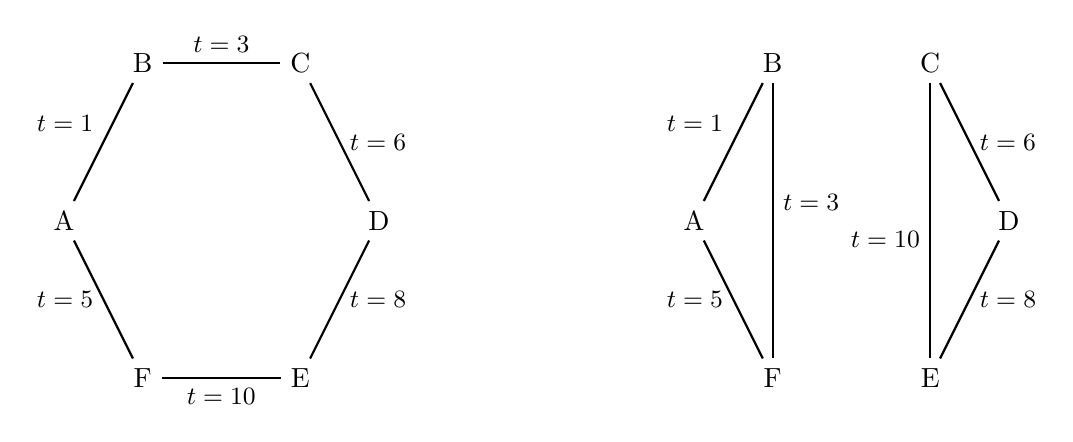
\begin{tikzpicture}[-, >=latex, node distance=2cm, thick, scale = 1]
        % Nodes (Left Graph)
        \node (A) at (-5, 2) {A};
        \node (B) at (-4, 4) {B};
        \node (C) at (-2, 4) {C};
        \node (D) at (-1, 2) {D};
        \node (E) at (-2, 0) {E};
        \node (F) at (-4, 0) {F};

        % Edges before RE
        \path[every node/.style={font=\sffamily\small}]
        (A) edge node[above left] {$t=1$} (B)
        (B) edge node[above] {$t=3$} (C)
        (C) edge node[right] {$t=6$} (D)
        (D) edge node[right] {$t=8$} (E)
        (E) edge node[below] {$t=10$} (F)
        (F) edge node[left] {$t=5$} (A);

        % Nodes (Right Graph)
        \node (A') at (3, 2) {A};
        \node (B') at (4, 4) {B};
        \node (C') at (6, 4) {C};
        \node (D') at (7, 2) {D};
        \node (E') at (6, 0) {E};
        \node (F') at (4, 0) {F};

        % Edges after RE
        \path[every node/.style={font=\sffamily\small}]
        (A') edge node[above left] {$t=1$} (B')
        (B') edge node[above right] {$t=3$} (F')
        (C') edge node[right] {$t=6$} (D')
        (D') edge node[right] {$t=8$} (E')
        (E') edge node[below left] {$t=10$} (C')
        (F') edge node[left] {$t=5$} (A');
    \end{tikzpicture}
    \caption{An example of a single step in the RE procedure involves shuffling the edges \( BC \) and \( FE \) to \( BF \) and \( CE \), respectively, while maintaining their original time stamps.} \label{fig:re_stability}
\end{figure}

\iffalse
\begin{figure}[h!]
    \centering
    \begin{tikzpicture}[-, >=latex, node distance=2cm, thick]
        % Nodes (Left Graph)
        \node (A) at (-5, 2) {A};
        \node (B) at (-4, 4) {B};
        \node (C) at (-2, 4) {C};
        \node (D) at (-1, 2) {D};
        \node (E) at (-2, 0) {E};
        \node (F) at (-4, 0) {F};

        % Edges before RE
        \path[every node/.style={font=\sffamily\small}]
        (A) edge node[above left] {$3$} (B)
        (B) edge node[above] {$2.5$} (C)
        (C) edge node[right] {$2.5$} (D)
        (D) edge node[right] {$2$} (E)
        (E) edge node[below] {$3.5$} (F)
        (F) edge node[left] {$4.5$} (A);

        % Nodes (Right Graph)
        \node (A') at (3, 2) {A};
        \node (B') at (4, 4) {B};
        \node (C') at (6, 4) {C};
        \node (D') at (7, 2) {D};
        \node (E') at (6, 0) {E};
        \node (F') at (4, 0) {F};

        % Edges after RE
        \path[every node/.style={font=\sffamily\small}]
        (A') edge node[above left] {$3$} (B')
        (B') edge node[above right] {$2$} (F')
        (C') edge node[right] {$3$} (D')
        (D') edge node[right] {$2$} (E')
        (E') edge node[below left] {$3$} (C')
        (F') edge node[left] {$3$} (A');
    \end{tikzpicture}
    \caption{\centering{The associated clique complex before the RE step has one 
    connected component and a one dimensional feature, whereas the clique complex corresponding to the graph after the RE step has two connected components and no one dimensional features.}}
\end{figure}

Let $G'$ be a temporal graph obtained from $G$ by a single RE step by on the pair $(( u_1, v_1 ), (u_2, v_2,))$.
Let $G'_W = (V, E', f _{G'})$ and 
$G_f = (V, E, f _{G})$ be the corresponding weighted graphs.
For $e \in E \cap E'$, we have 

$$ | f _{G} (e) -  f _{G'} (e) |  \leq $$
$$ \frac{\sum_{e' \in \nedges(e)} \sum_{t_G \in \tim(e) , t'_G \in \tim(e')}| t_G - t'_G| - \sum_{e' \in \nedges(e)} \sum_{t_{G'} \in \tim' (e) , t'_{G'} \in \tim'(e')}| t_{G'} - t'_{G'}|}{|\nedges(e)|}  $$ 
$$ = \frac{\sum_{t \in Time_G(e), t_1 \in Time_G(u_1,v_1) }  |t - t_1| - \sum_{t \in Time_G(e), t_2 \in Time_G(u_1,v_2) }  |t - t_2| }{|\nedges(e)|} $$
$$ \leq \frac{\sum_{t_1 \in Time_G(u_1,v_1),t_2 \in Time_G(u_1,v_2) }| t_1 - t_2 |}{|\nedges(e)|} $$
$$ \leq max {|t_1 - t_2 |} $$


Eventough we cannot guarentee sability, we claim that for some 
$\alpha \in \mathbb{R}$, apart from some $O (n)$ many peristance pairs, 
the RE procedure is stable where $n$ is the number of RE steps. 
This is due to that fact the perubation is localised, that is, for most edges $e \in E \cap E'$, $ f _{G} (e) = f _{G'} (e) $.


\paragraph*{DCWB Procedure}

In this method , we randomly select pair $(u_1,v_1), (u_2.v_2) \in V \times V$, such that 
$| \tim (u_1,v_1) | = | \tim (u_2,v_2) |$. The result is a graph where the time labels 
corresponding to the pairs $(u_1,v_1)$ and $(u_2,v_2)$ are interchanged.
This is done multiple times to construct a new graph.
The stability computation is similar to that of the RE procedure,

\paragraph*{CM Procedure}

Given a temporal graph $G$, we first consider a configuration model of $G$.
We then randomly assign all the time labels, and permute them further. 
This procedure completely destroys all temporal and structural information of the original 
graph. The D procedure is used to create a class of different graphs in the experiments.

More detailed analysis of these methords can be found in \cite{}.
\fi

%\newpage
\section{Experiments}\label{sec:experiments}
In this section, we present experiments to evaluate the effectiveness of our method in classifying temporal graphs.

\paragraph{\textbf{Method:}} We compute the average filtration for each temporal graph, from which we derive the persistence diagram (up to degree 2) based on the associated flag filtration. The Persistence Scale Space (PSS) kernel~\cite{reininghaus2015stable} is then used to compute the kernel distance matrix for each degree of the diagram, resulting in three matrices corresponding to degrees 0, 1, and 2. These matrices are combined with equal weights~\footnote{Different weights would allow for controlling the importance of each degree.} to produce a unified kernel matrix.

The combined kernel matrix is then utilized to train an SVM model for class prediction. All experiments were implemented in Python, with C++ used to compute the kernel matrices and the \( f_\mathrm{avg}^\mathrm{mlt} \) filtration for multi-labeled temporal graphs. The experiments were conducted on a server equipped with an Intel(R) Core(TM) i7-6950X CPU and dual NVIDIA GeForce RTX 2080 Ti GPUs to ensure consistent runtime and accuracy comparisons.

The datasets were divided into training and testing sets with an 80-20 split ratio, and accuracy was recorded on the testing set for each experiment. The accuracy score was calculated as the ratio of correctly predicted data points to the total number of data points. The source code is publicly available\footnote{ \href{https://github.com/phtgraph/temporal_classification?tab=readme-ov-file} {Source Code Repository Link.}}.



\paragraph{\bf{Datasets}:} The datasets used in the first two experiments are contact sequence datasets. The first dataset is a real-world dataset from the SocioPatterns dataset repository~\cite{sociopatterns_datasets}. %We have used the Hospital Ward~\cite{hospital_data} and High-School~\cite{highschool} dynamic contact network datasets, Workplace contacts~\cite{workplacev2} dataset and a temporal network of student contacts at MIT~\cite{Eagle2006}. 
The second dataset is synthetic and is generated using the model described in~\cite{Holme2012}. In the last two experiments (Pure and Mixed Classes), graphs are randomly generated and do not model any specific phenomena. For real datasets, typically, only a single temporal graph is available, whereas synthetic datasets can provide one or more initial graphs, termed \textbf{root graphs}. Classes are created as described in Section~\ref{sec:Stability}. The TP, EWLSS, and RE procedures generate loosely similar graphs, while the CM procedure produces distinct ones. With a single root graph, two classes are formed: one with loose copies of the root graph and another with multiple CM-generated graphs. For multiple root graphs, classes are formed by loosely copying each root graph.

We begin with experiments on contact sequence datasets, followed by additional tests on randomly generated temporal graphs.


\subsection{Contact Sequence Datasets}

%We perform experiments on the real contact dataset available on sociopattern data set.
%There are variety of temporal graphs, some are single labeled some are multi labled. 
%We also use different techniques to create classes, for example splitting the datasets in two different types as working hours and non-working hours. 
%We also used the null model techniques to create classe. \sid{Add more details here}

%These are multi-labelled temporal graphs. The primary approach used throughout is to start with a root graph and then create classes for the classification task using techniques described in Section~\ref{sec:Stability}. For example, given a root graph, one class could be created by applying the RE procedure to the root graph and another class could be created using the D procedure to the root graph. In cases where the dataset containts two root graphs (eg : HighSchool dataset) or where we are able to split the dataset into two different graphs (eg : Hospital dataset has been split into working and non-working hours), we use the same procedure for both the classes. The avg accuracy (over 5 runs) for the experiments have been descirbed in Table~\ref{tab:combined_average}.
All temporal graphs in the following experiments (Table~\ref{tab:combined_average_real_contact} and Table~\ref{tab:combined_averages_synthetic_contact}) are multi-labeled and we use $f_\mathrm{avg}^\mathrm{mlt}$ filtration as described in Section~\ref{sec:temp_filtration}.

\paragraph{\bf{Real Datasets:}} All experiments involve two classes. In the \emph{Class Generation} column (Table~\ref{tab:combined_average_real_contact}), RE+CM denotes that the first class of similar temporal graphs is generated via the RE procedure, while the second, dissimilar class is created using the CM procedure. Other symbols follow the same convention. Except for the Hospital (Working/Non-Working) and HighSchool (2011/2012) experiments, all use a single root graph. In the Hospital experiment, the root graph is split into working and non-working hours, while in the HighSchool experiment, the split is based on contact years (2011 and 2012). For two-root datasets, the RE procedure is used to populate the two classes. Experiments on Hospital, MIT, and Workplace data (the first six experiments) employ different population methods, namely RE and EWLS for the similar classes. However, no significant difference in accuracy is observed. The general statistics for each dataset are provided in Table~\ref{tab:dataset_stats}.


\begin{table}[hpt]
\centering
%\resizebox{1\textwidth}{!}{
\begin{tabular}{|l|l|l|l|}
\hline
\textbf{Dataset}    & \textbf{Class Generation}   & \textbf{Accuracy} & \textbf{Stdev} \\ \hline
Hospital Combined          & RE+CM       & 0.98625                   & 0.01450                \\ \hline
Hospital Combined         & EWLS+CM        & 0.98625                   & 0.01575                \\ \hline
MIT     				& RE+CM         & 0.94375                   & 0.02990                \\ \hline
MIT     				& EWLS+ CM & 0.93875                   & 0.04000                \\ \hline
Workplace v2     				& RE+CM         & 1                   & 0                \\ \hline
Workplace v2     				& EWLS+ CM   & 1                   & 0                \\ \hline
Hospital (Working/Non-Working)   & RE+RE       &  0.925          & 0.02500           \\ \hline
HighSchool 2011       & RE + CM  & 1 & 0. \\ \hline
HighSchool 2012       & RE + CM   & 1 & 0 \\ \hline
HighSchool (2011/2012)   & RE+RE  & 0.9866 & 0.04604 \\ \hline

\end{tabular} %}
\caption{{Combined averages of accuracy and standard deviation across different datasets. 
}}
\label{tab:combined_average_real_contact}
\end{table}

\begin{table}[ht]
    \centering
    %\resizebox{1\textwidth}{!}{
    \begin{tabular}{|l|l|l|l|l|l|l|l|}
        \hline
        \textbf{Dataset} & \textbf{$|V|$} & \textbf{$|E_s|$} & \textbf{$|E|$} & \textbf{$E_{avg}$} & \textbf{$E_{max}$} & \textbf{$d_{avg}$} & \textbf{$d_{max}$} \\ \hline
        Highschool 2011 & 126 & 1710 & 28540 & 16.69 & 1185 & 27.14 & 55 \\ \hline
        Highschool 2012 & 180 & 2220 & 45047 & 20.29 & 1280 & 24.67 & 56 \\ \hline
        Hospital Combined & 75 & 1139 & 32424 & 28.47 & 1059 & 30.37 & 61 \\ \hline
        MIT & 96 & 2539 & 234757 & 92.46 & 4387  & 52.9 & 92 \\ \hline
        Workplace v2 & 217 & 4274 & 78249 & 18.31 & 1302 & 39.39 & 84 \\ \hline
    \end{tabular} %}
    \caption{$|V|$ is the number of vertices, $|E_s|$ is the number of aggregate graph edges, $|E|$ is the number of temporal edges, $E_{\text{avg}}$ and $E_{\text{max}}$ are the average and maximum number of time labels per graph edge, and $d_{\text{avg}}$ and $d_{\text{max}}$ are the average and maximum temporal degree of the nodes.
}
    \label{tab:dataset_stats}
\end{table}

When classes are defined using the RE and EWLS procedures, they represent highly similar temporal graphs, making them inherently challenging to separate. This observation is confirmed in the following experiments (Table~\ref{tab:combined_average_real_contact_same_class}), validating our approach of defining classes based on reference models.

\begin{table}[ht]
    \centering
    %\resizebox{1\textwidth}{!}{
    \begin{tabular}{|l|l|l|l|}
    \hline
    \textbf{Dataset}    & \textbf{Class Generation}       & \textbf{Accuracy} & \textbf{Stdev} \\ \hline
    Hospital Combined          & RE + RE        & 0.5075                   & 0.08419               \\ \hline
    Hospital Combined         & EWLS + EWLS        & 0.5325                 & 0.06934               \\ \hline
    % Hospital (Working/Non-Working)   & RE+RE   & 75/1139       &  0.925          & 0.02500           \\ \hline
    HighSchool 2011       & RE + RE  & 0.45875 & 0.05338 \\ \hline
    HighSchool 2011       & EWLS + EWLS   & 0.505 & 0.07068 \\ \hline
    HighSchool 2012       & RE + RE  & 0.50625 & 0.05741 \\ \hline
    HighSchool 2012       & EWLS + EWLS  & 0.49625 & 0.05016 \\ \hline
    % HighSchool (2011/2012)   & RE+RE  & 306/3930 & 0.9866 & 0.04604 \\ \hline
    % MIT     				& RE+D      &  96/2539      & 0.94375                   & 0.02990                \\ \hline
    % MIT     				& EWLS+ D   & 96/2539  & 0.93875                   & 0.04000                \\ \hline
    % Workplace v2     				& RE+D      &  217/4274      & 1                   & 0                \\ \hline
    % Workplace v2     				& EWLS+ D   & 217/4274  & 1                   & 0                \\ \hline
    \end{tabular} %}
    \caption{{Combined averages of accuracy and standard deviation across different datasets using same root graph for both classes.}}
    \label{tab:combined_average_real_contact_same_class}
    \end{table}

\subparagraph*{\bf{Synthetic Dataset:}} 
We generate three root temporal graphs with varying parameters using both \textit{disassortative} and \textit{assortative} mixing strategies, as described in \cite{Holme2012}. These multi-labeled temporal graphs model contact and disease transmission dynamics. The last two experiments use the same set of graphs: in the third experiment, we include all points from the persistence diagram, while in the fourth, we use a pruned persistence diagram, removing low-persistence points. We observed a minimal drop in accuracy, while the runtime decreased by nearly half.

\begin{table}[h!]
\centering
%\resizebox{1\textwidth}{!}{
\begin{tabular}{|l||c|c|c|c|}
\hline
\textbf{Class} & \textbf{|V|/|E|} & \textbf{Threshold}   & \textbf{Average Accuracy} & \textbf{Average Stdev} \\ \hline
3 & 100/200               & 0   & 0.9733                    & 0.0235 \\ \hline
3 & 250/500               & 0   & 1.0000                   & 0.0000  \\ \hline
3 & 100/1000              & 0   & 0.9681 (104s) 				  &  0.0283   \\ \hline
3 & 100/1000              & 300 & 0.9385 (49s)				  & 0.0396     \\ \hline
\end{tabular} %}
\caption{In the first two experiments, we use 18 distinct parameter sets, while in the last two, we use 6. For each parameter set, the average result is reported over 5 runs. On average, 20 RE steps were performed to generate a new class member in the first two experiments, compared to 32.5 RE steps in the last two. The runtime for the third and fourth experiments is 104 seconds and 49 seconds, respectively.
 %The mixing functions take 2 parameters to decide if 2 nodes become a pair, $x_i$ which sets the strength of assortativity or disassortativity and $d_{max}$ is the maximum degree a node can take in a graph. 
}
\label{tab:combined_averages_synthetic_contact}
\end{table}

%The last two experiments are done on same set of graphs. However, we performed the third experiment with the complete persistence diagram and the fourth with a  pruned (removal of low persistence points) persistence diagram. With these two experiments we wanted to compare the accuracy versus the efficiency after pruning the PD. We observed very little drop in accuracy however time taken to perform the whole experiment dropped by nearly a factor of 2.

\iffalse
\begin{table}[h!]
    \begin{tabular}{|c|c|c|c|c|c|c|}
    \hline
    \textbf{$G_1$ parameters} & \textbf{$G_2$ parameters} & \textbf{$G_1$ parameters} & \textbf{RE changes} & \textbf{Threshold} & \textbf{Accuracy} & \textbf{Time} \\ \hline
    (0.7, 0.2, D) & (0.7, 0.2, D) & (0.7, 0.2, D) & 25 & 0 & 1.0 & 104.22 \\ \hline
    (0.7, 0.2, D) & (0.7, 0.2, D) & (0.7, 0.2, D) & 25 & 300 & 0.9967  & 48.06 \\ \hline
    (0.7, 0.2, D) & (0.7, 0.2, D) & (0.7, 0.2, D) & 50 & 0 & 0.94  & 104.98 \\ \hline
    (0.7, 0.2, D) & (0.7, 0.2, D) & (0.7, 0.2, D) & 50 & 300 & 0.8967 & 52.13 \\ \hline
    (0.7, 0.2, A) & (0.7, 0.2, A) & (0.7, 0.2, A) & 25 & 0 & 1.0 & 103.77 \\ \hline
    (0.7, 0.2, A) & (0.7, 0.2, A) & (0.7, 0.2, A) & 25 & 300 & 1.0 & 46.51 \\ \hline
    (0.7, 0.2, A) & (0.7, 0.2, A) & (0.7, 0.2, A) & 50 & 0 & 0.93  & 101.05 \\ \hline
    (0.7, 0.2, A) & (0.7, 0.2, A) & (0.7, 0.2, A) & 50 & 300 & 0.89  & 48.56 \\ \hline
    (0.7, 0.2, A) & (0.7, 0.2, D) & (0.7, 0.2, A) & 25 & 0 & 1.0 & 102.62 \\ \hline
    (0.7, 0.2, A) & (0.7, 0.2, D) & (0.7, 0.2, A) & 25 & 300 & 0.9967  & 48.58 \\ \hline
    (0.7, 0.2, A) & (0.7, 0.2, D) & (0.7, 0.2, A) & 50 & 0 & 0.9433  & 103.85 \\ \hline
    (0.7, 0.2, A) & (0.7, 0.2, D) & (0.7, 0.2, A) & 50 & 300 & 0.8767  & 48.7 \\ \hline
    \end{tabular}
    \label{tab:exp4-thresh}
    \caption{\centering{Exp 3 : (V,E)=(100,1000), $(x_i,d_{max})=(0.5,30)$, with persistence threshold}}
    \end{table}
\fi

\subsection{Random Temporal Graphs} 
%In Figures~\ref{fig:random_plot1} and~\ref{fig:random_plot2}, we present the results of our experiments on random temporal graphs. Both experiments use single-labeled graphs and the $f_\mathrm{avg}$ filtration, as described in Section~\ref{sec:temp_filtration}. The goal is to assess the effectiveness of our approach with a large number of similar classes and to evaluate its performance under varying temporal graph sparsity. To generate different classes, we apply the TP procedure from Section~\ref{sec:Stability} to a fraction of interactions, referred to as \textit{out shifts}. For a single class, the TP procedure is applied to a smaller fraction of edges, referred to as \textit{in shifts}. More details of this strategy are provided for each experiment.
Figures~\ref{fig:random_plot1} and~\ref{fig:random_plot2} show the results of experiments on random temporal graphs using single-labeled graphs and the $f_\mathrm{avg}$ filtration described in Section~\ref{sec:temp_filtration}. These experiments evaluate our method's effectiveness with a large number of similar classes and mixed classes and its performance under varying temporal graph sparsity. Class generation employs the TP procedure from Section~\ref{sec:Stability}, applied to a fraction of interactions (\textit{out shifts}), while \textit{in shifts} apply TP to a smaller fraction of edges within a single class. Details of this strategy are provided for each experiment.

 
\subparagraph*{\bf{Pure Classes:}}
To create a homogeneous pool of classes, we generated a single-labeled temporal graph $G$ with 100 vertices and varying sparsity (0.05 to 0.8), with time stamps in the range $(0,100]$. For each experiment, the original root graph was used to create 3, 5, 7, or 9 new root graphs (classes) by shifting the time stamps (out-shifts) of an average of 4.75\% of interactions by $1 \leq \epsilon \leq 5$. To populate graphs within the same class, time stamps of an average of 1.6\% of interactions were shifted (in-shifts) by $1 \leq \epsilon \leq 5$.



% A single labeled temporal graph $G$ with 100 vertices and \sid{$e$ how many?} interactions was randomly generated.    Each edge had weights in the range $(0,100]$.    We then create $n$ root graphs $G_1,\dots,G_n$ using TP Procedure.   For each root graph, a class is created using the TP procedure, but on a smaller percentage of intractions.
    
%We provide accuracy results for temporal graphs across various sparcity in 
%Tables~\ref{tab:exp1-0.05},~\ref{tab:exp1-0.1},~\ref{tab:exp1-0.2},~\ref{tab:exp1-0.4}
%and ~\ref{tab:exp1-0.8}.

\begin{figure}[h!]
\centering
\begin{minipage}{0.5\textwidth} % Left minipage for the plot
    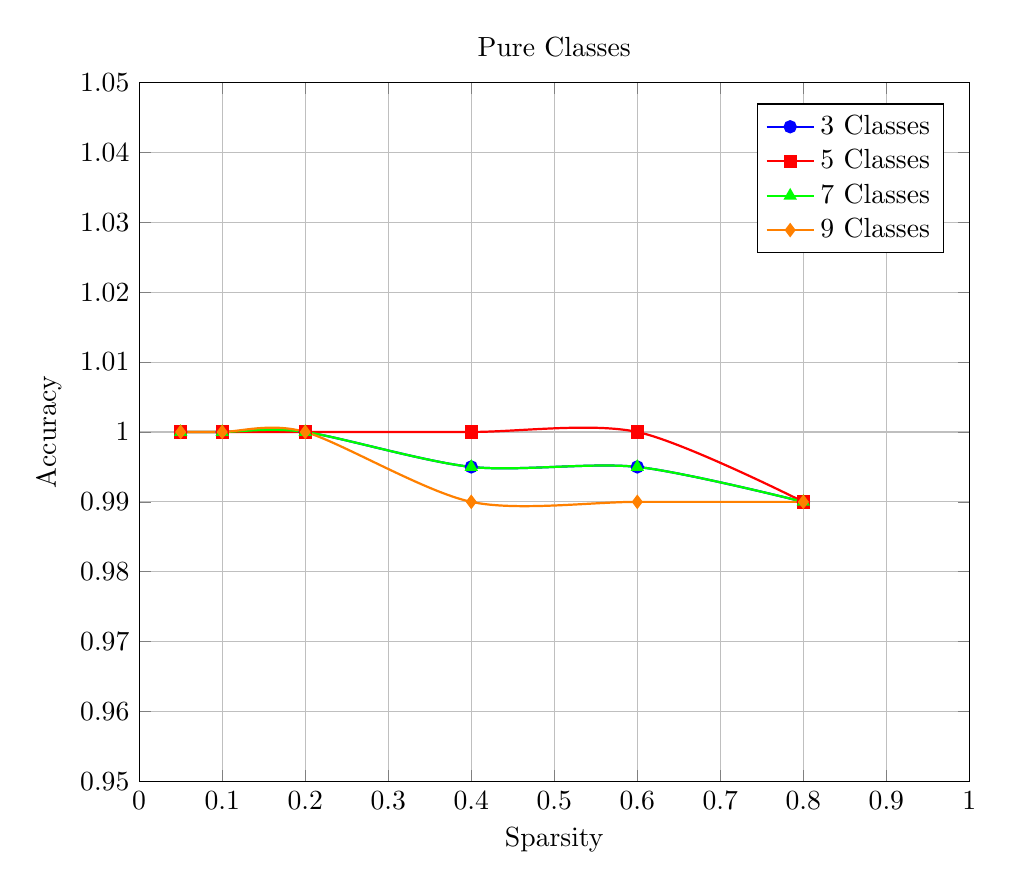
\begin{tikzpicture}
    \begin{axis}[
            width=1.0\textwidth,
            title={Pure Classes},
            xlabel={Sparsity},
            ylabel={Accuracy},
            xmin=0, xmax=1,
            ymin=0.95, ymax=1.05,
            legend pos=north east,
            grid=both,
            every axis plot/.append style={thick},
            cycle list={
                {blue,mark=*},
                {red,mark=square*},
                {green,mark=triangle*},
                {orange,mark=diamond*}
            }
        ]
    \legend{3 Classes , 5 Classes, 7 Classes, 9 Classes}    
    % Data points for Class 3
    \addplot[
        color=blue,
        mark=*,
        mark options={fill=blue},
        smooth
    ] coordinates {
        (0.05, 1.00)
        (0.1, 1.00)
        (0.2, 1.00)
        (0.4, 0.995)
        (0.6, 0.995)
        (0.8, 0.99)
    };

    % Data points for Class 5
    \addplot[
        color=red,
        mark=square*,
        mark options={fill=red},
        smooth
    ] coordinates {
        (0.05, 1.00)
        (0.1, 1.00)
        (0.2, 1.00)
        (0.4, 1.00)
        (0.6, 1.00)
        (0.8, 0.99)
    };

    % Data points for Class 7
    \addplot[
        color=green,
        mark=triangle*,
        mark options={fill=green},
        smooth
    ] coordinates {
        (0.05, 1.00)
        (0.1, 1.00)
        (0.2, 1.00)
        (0.4, 0.995)
        (0.6, 0.995)
        (0.8, 0.99)
    };

    % Data points for Class 9
    \addplot[
        color=orange,
        mark=diamond*,
        mark options={fill=orange},
        smooth
    ] coordinates {
        (0.05, 1.00)
        (0.1, 1.00)
        (0.2, 1.00)
        (0.4, 0.99)
        (0.6, 0.99)
        (0.8, 0.99)
    };

    \end{axis}
    \end{tikzpicture}
\end{minipage}%
\hfill % Creates horizontal space between the plot and the text
\begin{minipage}{0.4\textwidth} % Right minipage for the text
For each class and sparsity pair, we ran four experiments with different out- and in-shift combinations, and the results for each combination were averaged over 5 runs. %The plot shows the relationship between accuracy and sparsity for different numbers of classes (3, 5, 7, and 9). 
As the sparsity increases, the accuracy remains stable around 1.0 for all classes, with only minor drops at higher sparsity values. 
This indicates that the classification models maintain high performance even with lower data density.
%Variations in accuracy are minimal, especially for  5, 7, and 9 classes, with small fluctuations as sparsity increases. 
\end{minipage}

\caption{Accuracy vs. sparsity for different number of pure classes.} \label{fig:random_plot1}
\end{figure}


\paragraph{\bf{Mixed Classes:}} For mixed sets of classes, we used two single-labeled temporal graphs $G$, each with 100 vertices and varying sparsity (0.05 to 0.8) and time stamps in the range $(0,100]$. This setup enabled the creation of both similar and distinct class sets. For instance, Class $2$-$2$ consists of two classes from one root graph and its out-shifted variant, and two classes from a second root graph and its out-shifted variant. Similarly, Classes $2$-$3$ and $3$-$3$ were generated. Out-shifts affected an average of 4.75\% of interactions by $1 \leq \epsilon \leq 5$, while in-shifts altered an average of 1.88\% of interactions within the same range.



%We generate two single labeled temporal graphs $G$ and $G'$  100 vertices and $e$ interactions randomly. We then created $n$ root of graphs $G_1,\dots,G_n$ and $m$ root graphs $G'_1,\dots,G'_m$ using the TP procedure on $G$ and $G'$ respectively. Each class is then created using the TP procedure, but on a smaller percentage of interactions.

%We provide accuracy results for temporal graphs across various sparcity in 
%Tables~\ref{tab:exp3-0.2}, ~\ref{tab:exp3-0.4}, ~\ref{tab:exp3-0.6}, ~\ref{tab:exp3-0.8},
% ~\ref{tab:exp3-0.1} and \ref{tab:exp3-0.05}.

\begin{figure}[hpt]
    \centering
    \begin{minipage}{0.5\textwidth}
        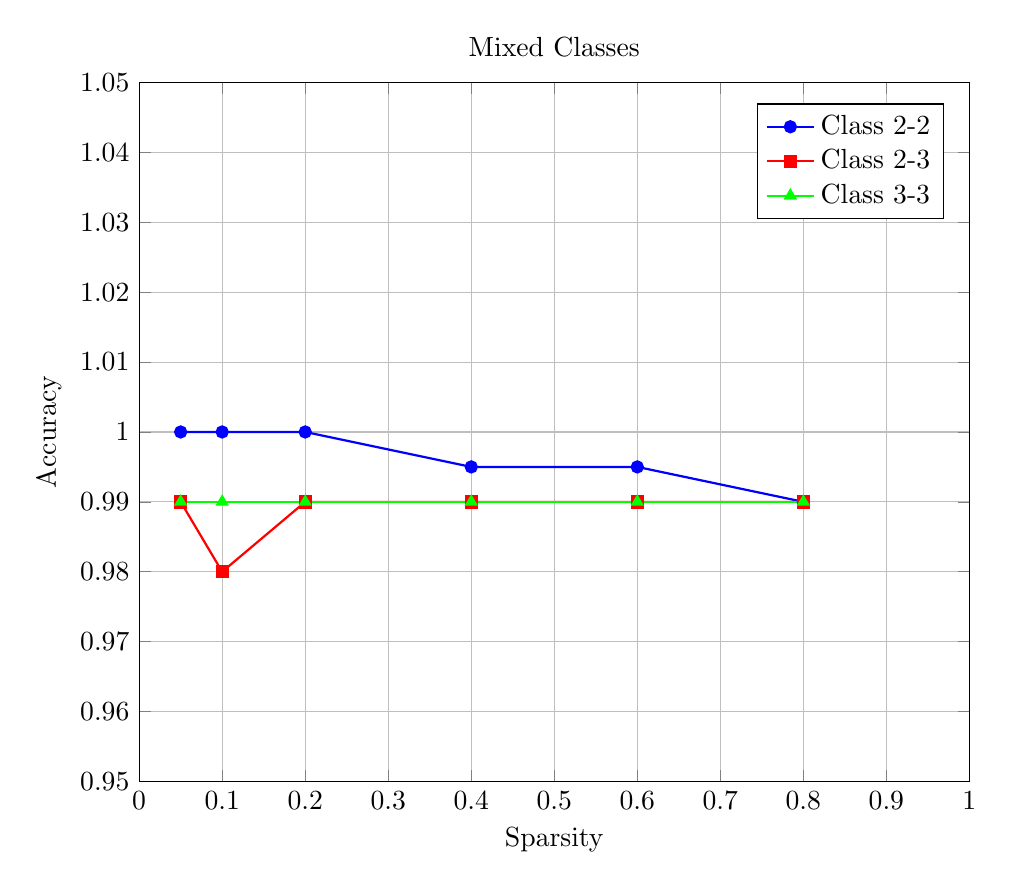
\begin{tikzpicture}
        \begin{axis}[
            width=1.0\textwidth,
            title={Mixed Classes},
            xlabel={Sparsity},
            ylabel={Accuracy},
            xmin=0, xmax=1,
            ymin=0.95, ymax=1.05,
            legend pos=north east,
            grid=both,
            every axis plot/.append style={thick},
            cycle list={
                {blue,mark=*},
                {red,mark=square*},
                {green,mark=triangle*},
                {orange,mark=diamond*}
            }
        ]

        % Data for Class 2-2
        \addplot coordinates {(0.05, 1.00) (0.1, 1.00) (0.2, 1.00) (0.4, 0.995) (0.6, 0.995) (0.8, 0.99)};
        
        % Data for Class 2-3
        \addplot coordinates {(0.05, 0.99) (0.1, 0.98) (0.2, 0.99) (0.4, 0.99) (0.6, 0.99) (0.8, 0.99)};
        
        % Data for Class 3-3
        \addplot coordinates {(0.05, 0.99) (0.1, 0.99) (0.2, 0.99) (0.4, 0.99) (0.6, 0.99) (0.8, 0.99)};
        
        \legend{Class 2-2, Class 2-3, Class 3-3}
        \end{axis}
        \end{tikzpicture}
    \end{minipage}
    \hspace{0.5cm}
    \begin{minipage}{0.35\textwidth}
For each class and sparsity pair, we conducted four experiments with different out- and in-shift combinations, averaging the results over five runs. The observed trends were consistent with the previous experiment (Figure~\ref{fig:random_plot1}), indicating that our classification model performs effectively in the mixed setup as well.

\end{minipage}
    \caption{Accuracy vs. sparsity for different number of mixed classes.}  \label{fig:random_plot2}
\end{figure}

\paragraph{\bf{Note:}} As noted in the Introduction, most temporal graph classification methods rely on node classes for classification~\cite{Micheli2022, Oettershagen2020}, whereas our approach does not. This difference prevents direct comparisons, as graph classes vary across studies.

However, to assess the inherent complexity of temporal graph classification and our pipeline's effectiveness, we experimented with the alternative minimum filtration and compared it to the average filtration. The results show that the average filtration performs better, leading us to select it for classification.


\subsection{Future Work} %We present a new approach to compute the persistent homology of temporal graphs using \(\delta\)-temporal motifs. The key innovation of our method lies in its ability to preserve temporal complexity without aggregation through discrete snapshots, offering a stable and efficient framework for temporal network analysis. This approach enables the computation of persistent homology on evolving graph structures, effectively capturing both local and global topological features. Moreover, our method is computationally efficient and scalable, with time and space complexity comparable to that of static graph methods.

%Experimentally, we demonstrate that our framework achieves over 92\% classification accuracy across diverse temporal graph datasets, all without requiring node classes. This node class free approach enhances its applicability, particularly in scenarios where node classes are unavailable or simulated. 

%Our framework has the potential to be extended to higher-order motifs, weighted edges, interval temporal graphs and probabilistic interactions, opening new avenues for research in dynamic systems. As shown here, the resulting persistence diagrams can be kernelized or vectorized, facilitating their application in standard machine learning tasks. This contributes to the integration of temporal graphs into the emerging field of Topological Machine Learning (TML), enhancing scalability and predictive power in areas such as epidemic modeling, social networks, and financial systems.
%We present a novel approach for computing the persistent homology of temporal graphs using $\delta$-temporal motifs. Our key innovation preserves temporal complexity without aggregating data into discrete snapshots, providing a stable and efficient framework for temporal network analysis. This enables the computation of persistent homology on evolving graph structures, capturing both local and global topological features. Additionally, our method is computationally efficient and scalable, with time and space complexity comparable to that of static graph methods.  

%Experimentally, we demonstrate that our framework achieves over 92\% classification accuracy across diverse temporal graph datasets, all without requiring node classes. This node-class-free approach enhances applicability, particularly in scenarios where node classes are unavailable or simulated.  

Our framework has the potential to be extended to higher-order motifs, weighted edges, interval temporal graphs, and probabilistic interactions, opening new research directions in dynamic systems. As shown, the resulting persistence diagrams can be kernelized or vectorized, enabling integration with standard machine learning tasks. This advances the role of temporal graphs in Topological Machine Learning (TML), enhancing scalability and predictive power in domains such as epidemic modeling, social networks, and financial systems.


\section*{Acknowledgement}
We thank Priyavrat Deshpande, Writika Sarkar, Mohit Upmanyu, and Shubhankar Varshney for their valuable input during the early discussions of the project.

\section*{Funding}
All three authors received partial support from a grant provided by Fujitsu Limited. Part of this work was carried out during the first author's visit to The University of Newcastle, NSW, Australia, and was partially funded by an ARC Discovery Grant (Grant Number: G2000134).

%\newpage
%\bibliographystyle{plainnat}
\bibliographystyle{plain}
%\bibliographystyle{unsrtnat}
\bibliography{references}

\end{document}
